%Schriftgroesse, Layout, Papierformat, Art des Dokumentes
\documentclass[listof=totoc, 12pt, oneside, bibliography=totoc, a4paper, parskip=full+, final]{scrreprt} 

%Einstellungen der Seitenraender, Zeilenabstand
\usepackage[left=4cm,right=3cm,top=3cm,bottom=2cm,bindingoffset=0cm]{geometry}
\usepackage{setspace} 
\setlength{\footskip}{0.8cm}

%Deutsche Rechtschreibung
\usepackage[ngerman]{babel}
\usepackage[babel,german=quotes]{csquotes}
\usepackage{mathptmx}

%BiblatexStyle
\bibliographystyle{unsrt}

%Umlaute ermoeglichen
\usepackage[utf8]{inputenc}
\usepackage[T1]{fontenc}
\usepackage{lmodern}
\usepackage{textcomp}

%Fuer Grafiken
\usepackage{graphicx} 
\usepackage{subfigure}
\usepackage{wrapfig}

%Fuer Tabellen
\usepackage{tabularx}
\usepackage{longtable}
\usepackage{array}

%Mathematische Zeichen
\usepackage{amsmath, amsthm, amssymb}
\usepackage{mathtools}

%Bildunterschriften
\usepackage{caption}
\addto\captionsngerman
{
	\renewcommand{\figurename}{Abb.}
	\renewcommand{\tablename}{Tab.} 
}

%Für Quellcode
\usepackage{listings}
\usepackage{color}
\definecolor{darkblue}{rgb}{0,0,.6}
\definecolor{darkred}{rgb}{.6,0,0}
\definecolor{darkgreen}{rgb}{0,.6,0}
\definecolor{lightblue}{rgb}{0.97,0.99,1}

\renewcommand{\lstlistingname}{Codeauszug}
\lstset
{
	basicstyle=\ttfamily\small,
	commentstyle=\color{darkgreen},
	keywordstyle=\bfseries\color{darkblue},
	stringstyle=\color{darkred},
	showspaces=false,
	showstringspaces=false,
	showtabs=false,
	columns=fixed,
	frame=single,
	frameround=ffff,
	numbers=left,
	numberstyle=\tiny,
	numbersep=5pt,
	breaklines=true,
	backgroundcolor=\color{lightblue},
	captionpos=b
}

%lädt das Paket zum erzwingen der Grafikposition
\usepackage{here} 

%Um Links im Dokument zu aktivieren
\usepackage{hyperref}
\hypersetup{
	colorlinks=false,
	pdfborder={0 0 0},
}

%Header and Footer - simplified
\usepackage{fancyhdr}
\pagestyle{fancy}
\fancyhf{}
\fancyfoot[C]{Mobile Computing Final Report - LogChirpy \quad \thepage}
\fancyhead[C]{\leftmark}
\renewcommand{\headrulewidth}{0.4pt}
\renewcommand{\footrulewidth}{0.4pt}

%Autor und Titel
\author{Martin Lauterbach, Luis Wehrberger, Youmna Samouneh}
\title{LogChirpy - Ornithological Archival App}

\begin{document}
\pagestyle{plain}

\pagenumbering{gobble}
%Deckblatt
\begin{titlepage}

\begin{center}

\begin{figure}
\begin{minipage}[H]{6cm}
\centering
\includegraphics[width=0.8\linewidth]{img/university_logo}
\end{minipage}
\hfill
\begin{minipage}[H]{6cm}
\centering
% Company/Project logo placeholder
\textbf{\Large LogChirpy}
\end{minipage}
\end{figure}

\vspace*{0.8cm}

\textbf{Hochschule Reutlingen Fakultät Informatik}\\
\textbf{Mobile Computing Project"} \\
\vspace*{0.2cm}
{\large \textbf{SoSe 2025\\}}
\vspace*{0.4cm}
Prof. Dr. Martinez\\
\vspace*{0.8cm}
{\large \textbf{- Final Report -}}

\textbf{{\large {\LARGE LogChirpy - Ornithological Archival App}}}\\
\textbf{{\large Bird Watching Application with AI-Powered Recognition}}\\

\noindent\rule{\textwidth}{2pt}
\vspace*{0.6cm}

\textbf{vorgelegt von:\\}
{\large \textbf{Martin Lauterbach\\}}
{\large \textbf{Luis Wehrberger\\}}
{\large \textbf{Youmna Samouneh\\}}

\vspace*{0.6cm}

Contact addresses:\\
martin.lauterbach@student.reutlingen-university.de\\
luis.wehrberger@student.reutlingen-university.de\\
youmna.samouneh@student.reutlingen-university.de\\

\vspace*{0.6cm}

Submitted on: \today

\vspace*{1cm}

\textbf{Abstract}\\
\vspace*{0.3cm}
\begin{minipage}{0.8\textwidth}
\small
This research presents LogChirpy, a comprehensive mobile ornithological documentation application developed using React Native and Expo frameworks. The application implements advanced artificial intelligence methodologies for automated avian species identification through integrated visual and acoustic analysis systems. The architecture employs local machine learning models for real-time species recognition, coupled with a sophisticated archival framework that supports both offline operation and optional cloud synchronization capabilities. The system incorporates multilingual functionality across six languages and maintains a comprehensive taxonomic database encompassing over 30,000 global avian species. LogChirpy addresses the requirements of both amateur naturalists and professional ornithologists by providing an intuitive platform for systematic documentation and collaborative sharing of ornithological observations.
\end{minipage}

\end{center}

\end{titlepage}

%Inhaltsverzeichnis
\cleardoublepage
\tableofcontents

%Abbildungsverzeichnis
\cleardoublepage
\listoffigures

%Tabellenverzeichnis
\cleardoublepage
\listoftables

\pagenumbering{arabic}
\pagestyle{fancy}
\cleardoublepage

%Kapitel 1 - Einführung und Motivation
\cleardoublepage
\chapter{Introduction}

Citizen-science bird monitoring generates observations at scales impossible for
professional ornithologists alone.
Platforms such as eBird receive hundreds of millions of observations annually,
yet data quality depends critically on observers' ability to identify species in
the field~\cite{Sullivan2009}.
Mobile applications with automated species recognition lower this barrier, but
most existing tools either require continuous network access, cover limited
geographic ranges, or rely on a single sensing modality.

BirdNET~\cite{BirdNET2021} demonstrated that a convolutional network trained on
spectrograms can achieve macro-averaged AUC $> 0.99$ across thousands of species,
making robust audio-based identification practical on consumer hardware.
Image-based classifiers such as MobileNetV2~\cite{Sandler2018} offer a
complementary modality; the two are rarely combined in an offline mobile context.

LogChirpy addresses three concrete gaps:

\begin{enumerate}
  \item \textbf{Multi-modal offline identification.}
        Combining BirdNET audio and a MobileNetV2 image classifier on-device,
        without any cloud inference dependency.

  \item \textbf{Large-scale multilingual reference database.}
        The Clements 2024 checklist~\cite{Clements2024} with 33,241 species
        in six languages and 9,331 Wikimedia Commons reference images, fully
        accessible offline.

  \item \textbf{Sequential pipeline architecture.}
        A unified service layer that eliminates the file-lock race conditions
        observed when audio recording and camera capture run concurrently on
        Android.
\end{enumerate}

The remainder of this paper describes the system architecture (Chapter~2),
an independent benchmark of the image classifier (Chapter~3), and a
discussion of limitations and scope (Chapter~4).


%Kapitel 2 - Ziele des Projekts
\cleardoublepage
\chapter{Project Objectives and System Requirements}

\section{Educational Development Goals}

\textbf{Learning Objectives:} Implementation of clear, discoverable navigation patterns with comprehensive user guidance and real-time feedback mechanisms, maintenance of uniform user experience and interface behavior across Android and iOS platforms while respecting platform-specific design conventions, minimization of onboarding complexity to enable rapid user adoption with progressive disclosure of advanced features, and comprehensive support for users with diverse accessibility requirements, adhering to WCAG guidelines and platform accessibility standards.

\textbf{Technical Quality Assurance Standards:} Implementation of well-documented, maintainable code following React Native best practices and industry standards, development of modular architecture facilitating straightforward maintenance, feature enhancement, and system evolution, implementation of thorough testing frameworks covering critical system components with automated validation protocols, and delivery of optimized performance across diverse device categories and hardware specifications.

\textbf{Security and Privacy Protection Framework:} Implementation of end-to-end encryption for user data during transmission and storage operations, full adherence to General Data Protection Regulation requirements with comprehensive privacy protection measures, prioritization of on-device ML processing to maximize data privacy and minimize external data exposure, and provision of user-controlled cloud synchronization features with granular privacy controls and data sovereignty options.



%Kapitel 3 - Anforderungsanalyse
\cleardoublepage
\chapter{Requirements Analysis and System Specification}


\section{Stakeholder Analysis and User Research}

\textbf{Primary Stakeholder Profile: Recreational Naturalist:}

\textbf{Demographic and Professional Characteristics:}
\begin{itemize}
    \item \textbf{Representative:} Professional software developer, age 35
    \item \textbf{Technical Proficiency:} Advanced digital literacy
    \item \textbf{Domain Experience:} Intermediate outdoor recreation and nature observation
    \item \textbf{Primary Activities:} Regular ecological excursions, wildlife photography, environmental documentation
    \item \textbf{Research Objectives:} Species identification enhancement, systematic observation logging, knowledge acquisition
    \item \textbf{Technical Challenges:} Taxonomic classification accuracy, data persistence, information management scalability
\end{itemize}

\textbf{Use Case Specification:} Automated Species Recognition and Documentation
\begin{quote}
As a recreational naturalist, the stakeholder requires a computational system capable of automated avian species identification through acoustic pattern recognition, enabling systematic documentation of field observations with integrated photographic evidence and geospatial coordinates within a persistent cloud-based archive.
\end{quote}

\textbf{Functional Requirements Specification:}
\begin{enumerate}
    \item The system shall provide accurate species identification through acoustic signal processing with validated confidence metrics
    \item The system shall support multimedia data capture and cloud synchronization for photographic evidence
    \item The system shall integrate GPS positioning services for precise geospatial documentation
    \item The system shall maintain persistent data storage with cross-platform accessibility through cloud infrastructure
\end{enumerate}

\textbf{Secondary Stakeholder Profile: Advanced Ornithological Practitioner:}

\textbf{Demographic and Professional Characteristics:}
\begin{itemize}
    \item \textbf{Representative:} Retired educational professional, age 50
    \item \textbf{Technical Proficiency:} Moderate digital adoption with learning willingness
    \item \textbf{Domain Experience:} Advanced ornithological knowledge and field experience
    \item \textbf{Primary Activities:} Systematic avian observation, conservation research, peer collaboration
    \item \textbf{Research Objectives:} Digital methodology adoption, comprehensive data management, professional knowledge sharing
    \item \textbf{Technical Challenges:} Traditional-to-digital workflow migration, data accuracy validation, large-scale information management
\end{itemize}

\textbf{Use Case Specification:} Comprehensive Digital Ornithological Platform
\begin{quote}
As an advanced ornithological practitioner, the stakeholder requires a sophisticated digital platform for species identification and systematic documentation, enabling efficient observation recording, comprehensive species data access, and collaborative research data exchange with the ornithological community.
\end{quote}

\textbf{Functional Requirements Specification:}
\begin{enumerate}
    \item The system shall provide professional-grade acoustic species identification with verifiable accuracy metrics
    \item The system shall support comprehensive observation documentation with multimedia evidence and precise geospatial data
    \item The system shall integrate extensive taxonomic databases with detailed species information and behavioral characteristics
    \item The system shall facilitate secure data exchange and collaboration mechanisms with authenticated ornithological practitioners
    \item The system shall maintain comprehensive data archival with long-term accessibility and cross-platform synchronization
\end{enumerate}

\section{Use Case Modeling and Validation}

\textbf{Use Case 1: Archive Access and Data Export Functionality:}
\textbf{Specification:} Multimedia Data Retrieval and External Platform Integration

\begin{quote}
The system shall provide recreational naturalists with intuitive archive navigation capabilities, enabling efficient multimedia content retrieval through advanced search functionality and seamless export integration with external applications, facilitating social media engagement and community knowledge sharing.
\end{quote}

\textbf{Acceptance Criteria and System Requirements:}
\begin{enumerate}
    \item The system shall implement user-friendly archive interface navigation with minimal interaction complexity
    \item The system shall provide comprehensive search functionality with metadata-based filtering for efficient multimedia content discovery
    \item The system shall support cross-platform export capabilities with standardized file format compatibility
    \item The system shall maintain original multimedia quality standards throughout the export process
    \item The system shall ensure persistent cloud-based data storage with reliable accessibility across multiple devices
\end{enumerate}

\textbf{Use Case 2: Real-time Content Sharing and Collaboration:}
\textbf{Specification:} Immediate Multimedia Distribution for Professional Networks

\begin{quote}
The system shall enable advanced ornithological practitioners to rapidly access and distribute recently captured observational evidence through streamlined sharing mechanisms, facilitating immediate collaboration and knowledge dissemination within professional ornithological communities.
\end{quote}

\textbf{Acceptance Criteria and System Requirements:}
\begin{enumerate}
    \item The system shall provide immediate access to recently captured multimedia content through optimized caching mechanisms
    \item The system shall implement integrated sharing functionality directly from content viewing interfaces
    \item The system shall support multi-platform distribution channels including social media, email, and professional communication platforms
    \item The system shall preserve multimedia quality standards throughout the sharing process
    \item The system shall maintain comprehensive data persistence through cloud-based archival systems
\end{enumerate}

\textbf{Use Case 3: Geospatial Data Analysis and Location Intelligence:}
\textbf{Specification:} Species-specific Location Retrieval and Mapping


\section{Functional Requirements}

\begin{enumerate}
    \item \textbf{Audio Classification:} Process bird calls with ≥85\% accuracy in <5 seconds
    \item \textbf{Visual Recognition:} Detect and classify birds from camera images
    \item \textbf{Species Database:} Provide access to 33,000+ bird species with multilingual support
    \item \textbf{Observation Logging:} Record sightings with photos, audio, GPS, and notes
    \item \textbf{Data Management:} Store observations locally with optional cloud sync
    \item \textbf{Offline Operation:} Function completely without internet connectivity
\end{enumerate}

\section{Non-Functional Requirements}

\begin{enumerate}
    \item \textbf{Performance:} App startup <2 seconds, First Start Database under a Minute, UI response <1 second
    \item \textbf{Compatibility:} Android 8.0+ and iOS 12.0+
    \item \textbf{Storage:} Minimum 500MB available space for ML models and Birdex Encyclopedia
    \item \textbf{Privacy:} All ML processing on-device, no data transmission required
\end{enumerate}



%Kapitel 4 - Konzeptionelles Modell
\cleardoublepage
\section{System Architecture}
\label{sec:arch}

LogChirpy is built on React Native / Expo SDK~52 targeting Android (API\,29+) and
iOS.
Three service pillars — ML Processing, BirDex Encyclopedia, and Logging System —
share a common navigation shell built on Expo Router (Figure~\ref{fig:arch}).
All ML inference runs locally via \texttt{react-native-fast-tflite};
network access is limited to optional Firestore sync and first-run image download.

\begin{figure*}[t]
  \centering
  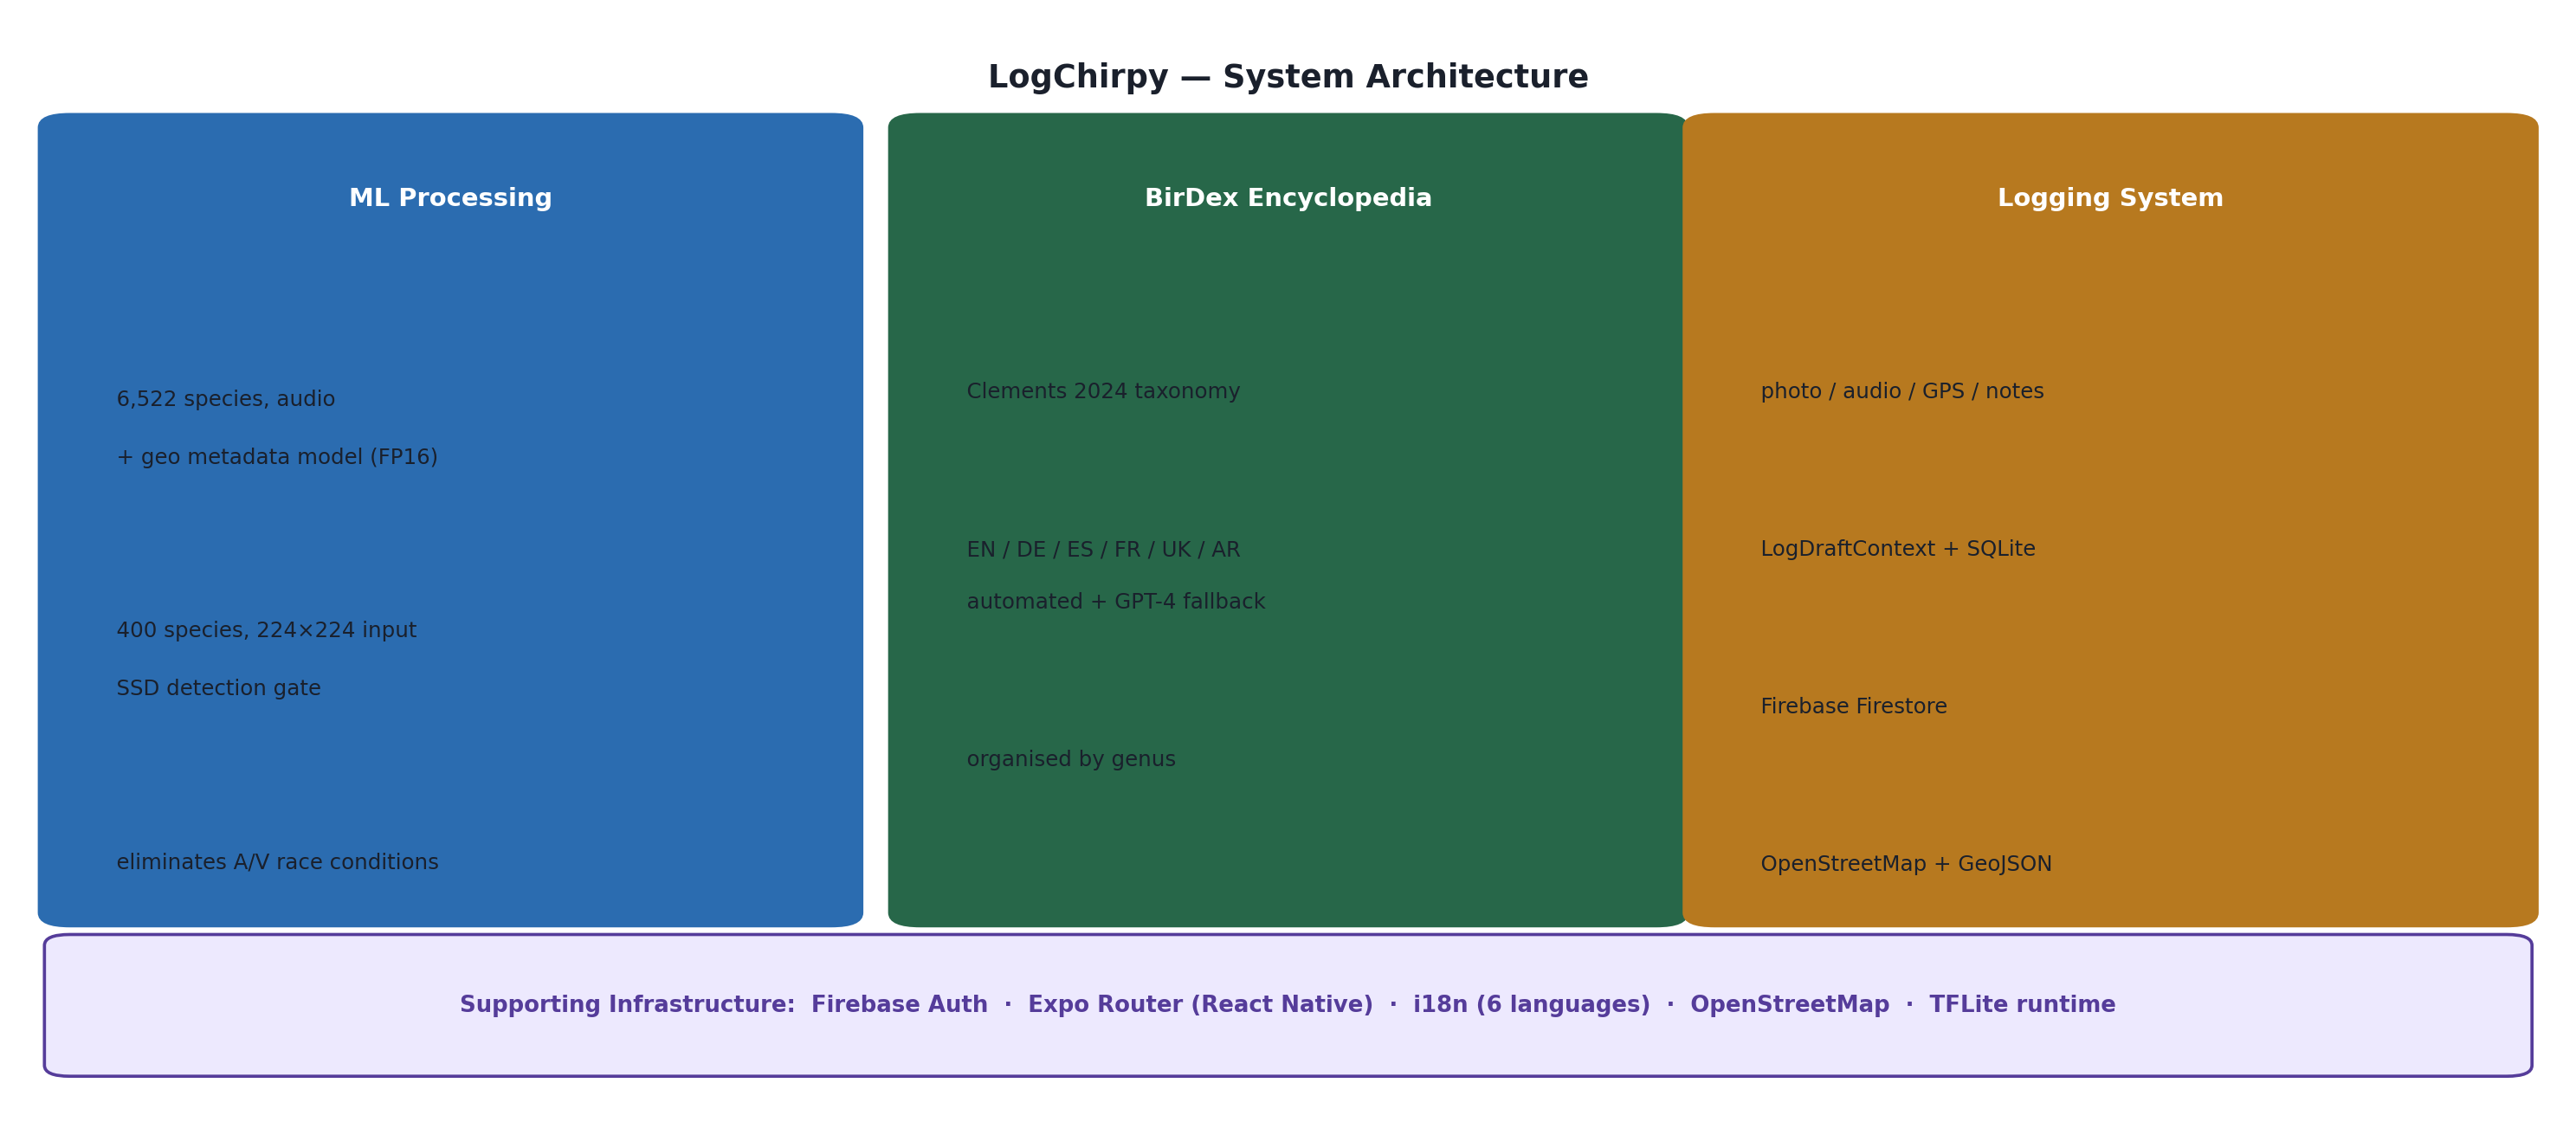
\includegraphics[width=\linewidth]{img/architecture.png}
  \caption{Three-pillar architecture. Each pillar is functionally independent;
           the unified sequential ML pipeline service (bottom bar) orchestrates
           audio and image processing to prevent Android file-lock conflicts.}
  \label{fig:arch}
\end{figure*}

\subsection{Audio Pipeline}

BirdNET\,v2.4~\cite{BirdNET2021} is implemented via two sequential TFLite models
(Figure~\ref{fig:pipelines}).
Audio is captured at 48\,kHz mono; a 150–15\,000\,Hz bandpass filter attenuates
wind and handling noise and the signal is normalised to $[-1,1]$.
The \textbf{acoustic model} (FP32) accepts a $\mathbb{R}^{1\times144\,000}$
tensor and outputs sigmoid logits over 6,522 species.
When GPS is available the \textbf{metadata model} (FP16) takes
$[\text{lat},\,\text{lon},\,\text{week-cos}]$ and produces a geographic prior;
scores are fused as
\begin{equation}
  p_{\text{blend}} = p_{\text{audio}}\cdot(0.7 + 0.3\cdot p_{\text{geo}}),
  \label{eq:blend}
\end{equation}
following the whoBIRD reference implementation~\cite{WhoBird2023}.

\subsection{Image Pipeline}

Camera frames are JPEG-compressed (quality\,0.3) and passed to an SSD MobileNet
V1 detection gate (MLKit).
Frames without a sufficiently confident bird detection are discarded.
Passing frames go to \texttt{bird\_classifier\_metadata.tflite}
(MobileNetV2~\cite{Sandler2018}): input $\mathbb{R}^{1\times224\times224\times3}$
normalised to $[-1,1]$, output softmax logits over 400 species.

\textbf{Sequential lock.}
Concurrent audio recording and camera processing caused
\texttt{MediaRecorder} file-lock conflicts on Android.
\texttt{unifiedMLPipelineService.ts} enforces image-before-audio sequencing,
eliminating all recorded stability errors.

\begin{figure*}[t]
  \centering
  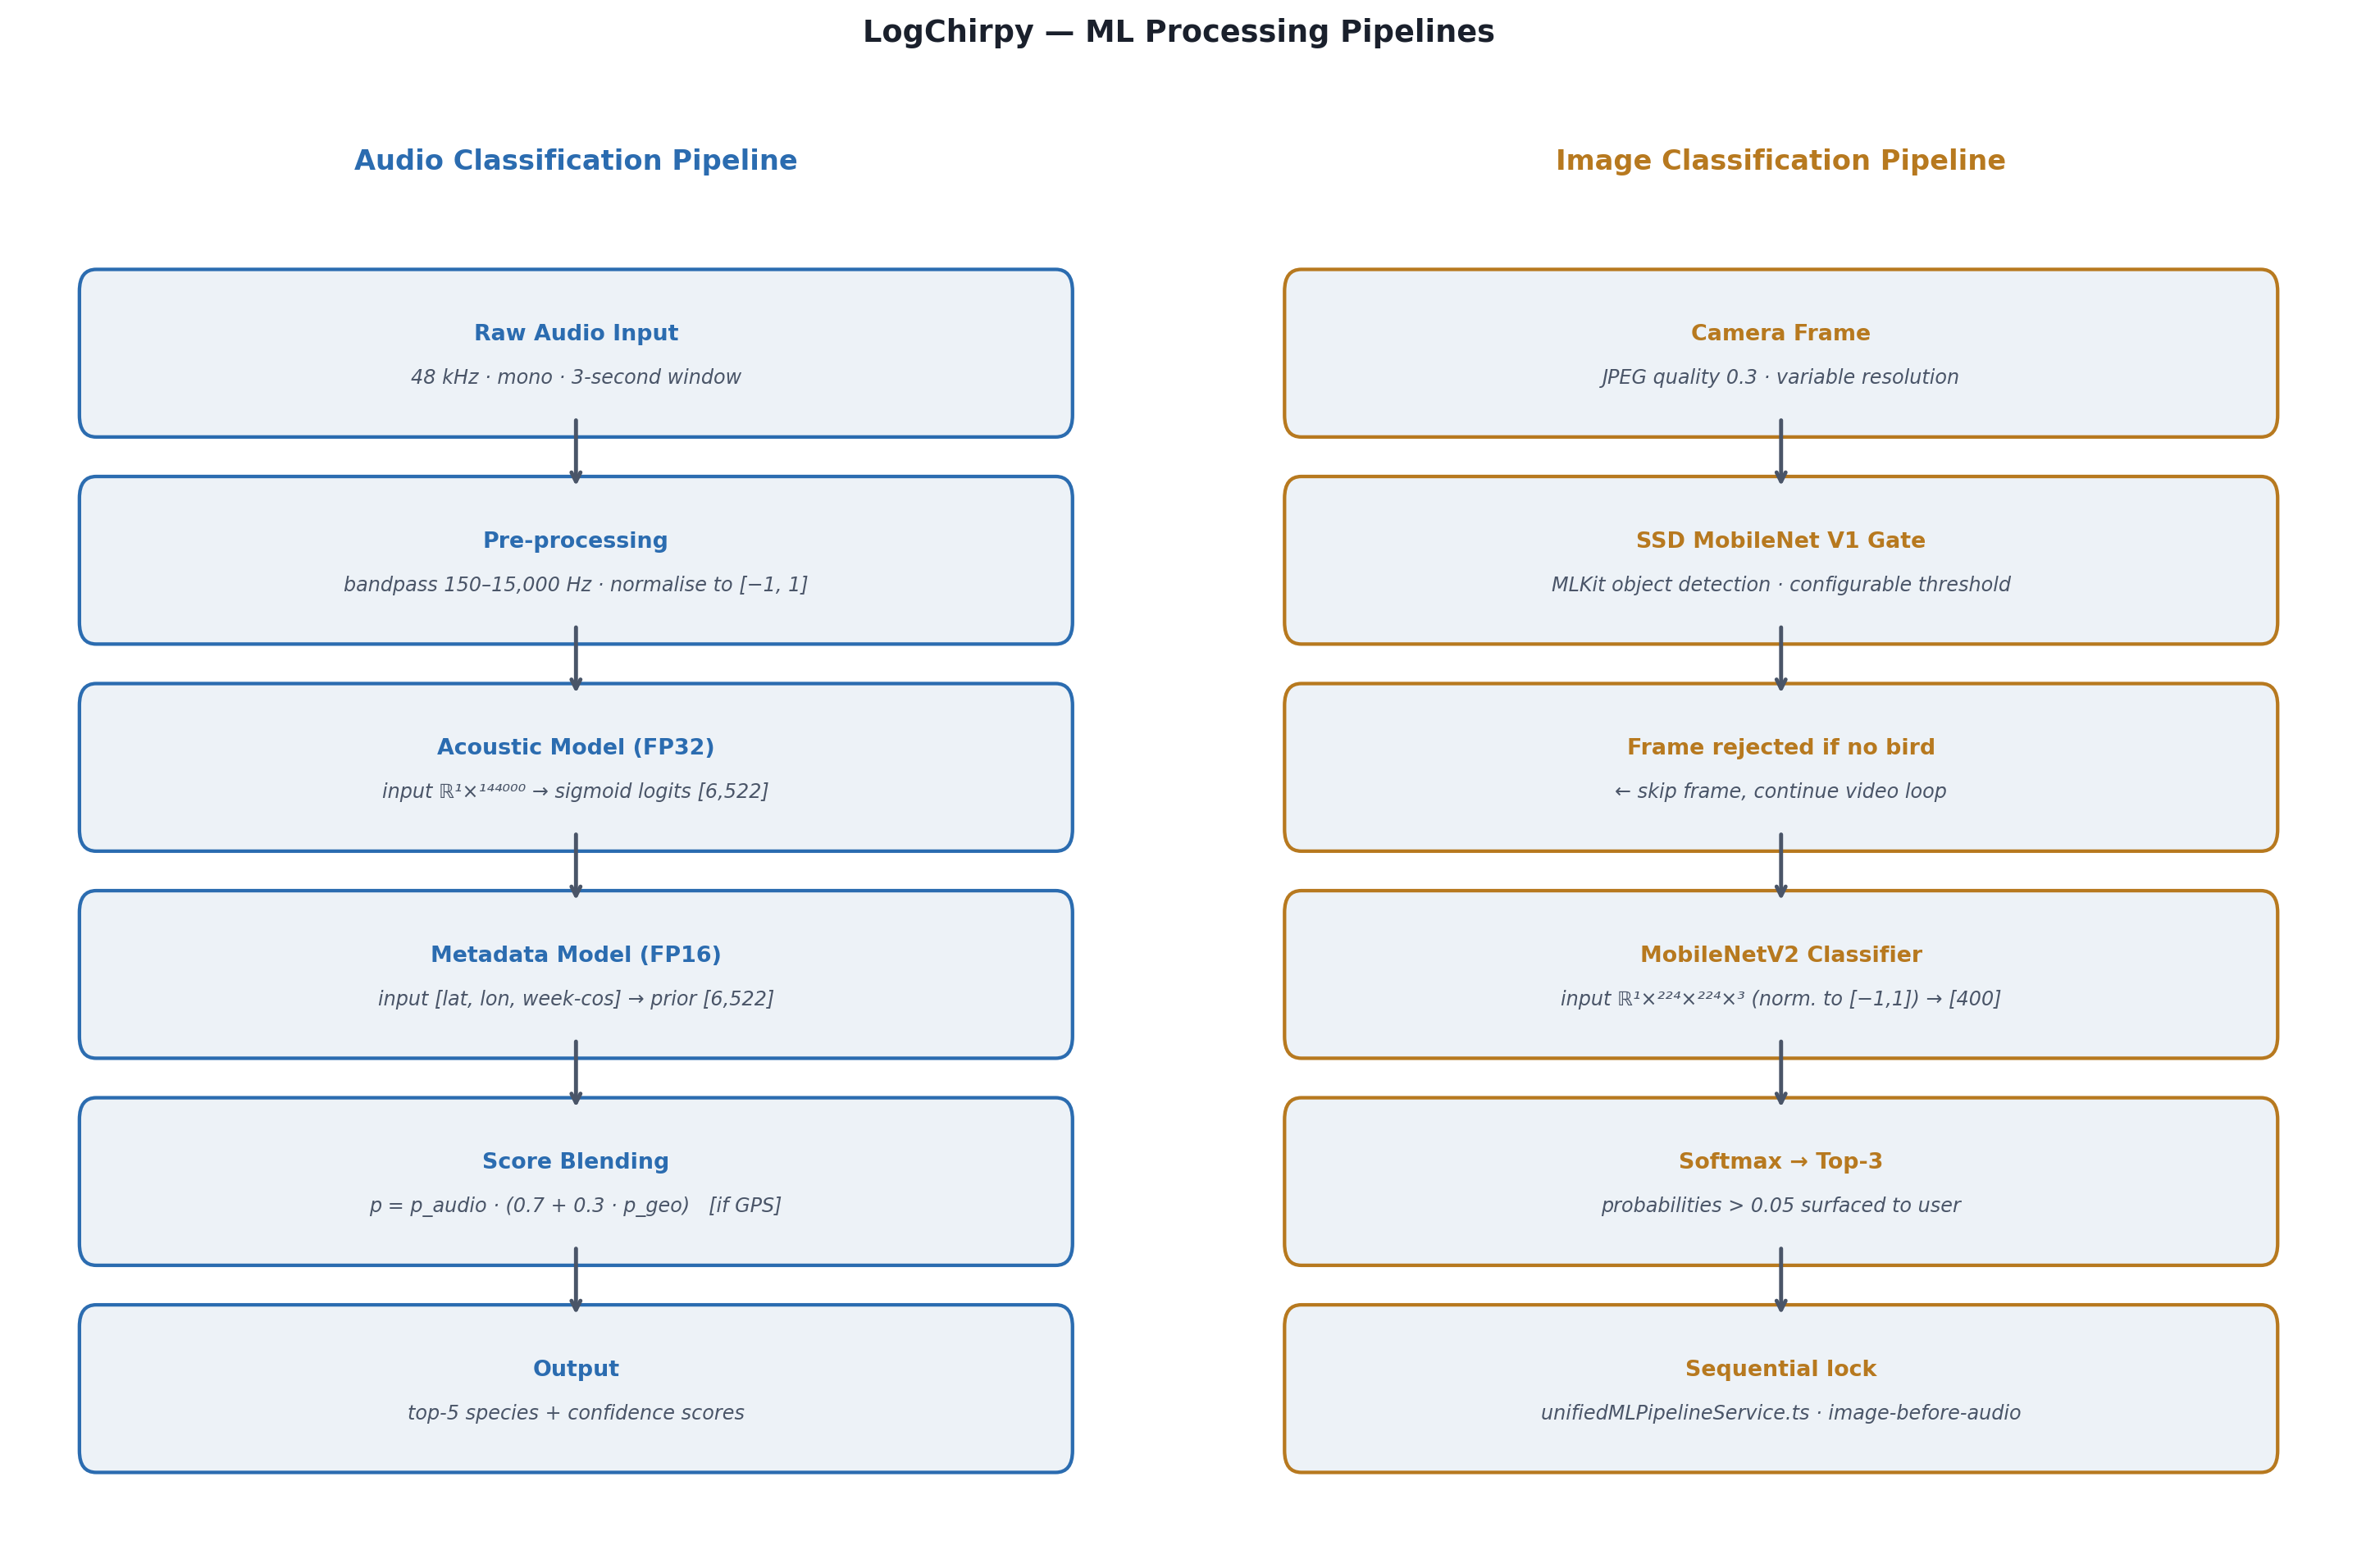
\includegraphics[width=\linewidth]{img/pipelines.png}
  \caption{Audio (left) and image (right) ML pipelines with tensor shapes.
           Both run entirely on-device via TFLite; the sequential lock prevents
           concurrent audio/camera conflicts on Android.}
  \label{fig:pipelines}
\end{figure*}

\subsection{BirDex Encyclopedia}

BirDex stores the complete Clements 2024 checklist~\cite{Clements2024} in an
on-device SQLite database (Table~\ref{tab:schema}).
Translations across six languages were generated by an automated pipeline
(DeepL\,$\to$\,Google Translate\,$\to$\,GPT-4 fallback) and spot-checked by
family.
Reference images (9,331 WebP files, $\approx$50\,kB each) are downloaded from
Wikimedia Commons at first launch and cached by Clements genus.

\begin{table}[htb]
\centering
\small
\setlength{\tabcolsep}{4pt}
\begin{tabular}{lll}
\hline
\textbf{Column} & \textbf{Type} & \textbf{Description} \\
\hline
\texttt{species\_code}    & TEXT PK & eBird 6-letter code \\
\texttt{english\_name}    & TEXT    & Clements English name \\
\texttt{scientific\_name} & TEXT    & Binomial nomenclature \\
\texttt{family / order}   & TEXT    & Clements taxonomy \\
\texttt{range}            & TEXT    & Breeding/wintering range \\
\texttt{de/es/fr/uk/ar}   & TEXT    & Translated names (×5) \\
\texttt{hasBeenLogged}    & INT     & Observation flag \\
\hline
\end{tabular}
\caption{BirDex SQLite schema (abridged, 33,241 rows).}
\label{tab:schema}
\end{table}


%Kapitel 5 - Design-Entscheidungen
\cleardoublepage
\chapter{Implementation Decisions and Development Process}

\section{Technology Selection and Rationale}

\textbf{React Native with Expo Framework}

React Native with Expo was selected for cross-platform development targeting both iOS and Android with a single codebase within the 12-week timeline.

Key benefits included hot reload for rapid development iterations and access to established ML libraries. ML model integration requirements necessitated transitioning from Expo Go to custom development builds.

The app architecture centers around tab-based navigation defined in \texttt{app/(tabs)/\_layout.tsx}, organizing features into six main sections: Home, BirDex, Archive, Gallery, Account, and Settings. The bird logging workflow is separated into dedicated screens under \texttt{app/log/}, including manual entry (\texttt{manual.tsx}), photo capture (\texttt{photo.tsx}), and AI-powered real-time detection (\texttt{objectIdentCamera.tsx}).

\textbf{Machine Learning Framework Selection}

Local ML processing was implemented for privacy considerations. TensorFlow Lite models and MLKit packages avoided cloud infrastructure and API costs within academic project constraints.

Existing models were adapted rather than training custom models due to time limitations and educational focus on mobile development. BirdNET models were converted from .h5 to .tflite format and integrated whoBIRD Kotlin implementation concepts through the \texttt{services/ultraSimpleBirdClassifier.ts} service.

\textbf{Database Architecture Approach}

Database design combines SQLite for local storage with Firebase Firestore for cloud synchronization. This hybrid approach was motivated by learning objectives to gain experience with both local and cloud database management.

The implementation consists of two main database services: \texttt{services/database.ts} manages bird observation records, while \texttt{services/databaseBirDex.ts} handles the 30,000+ species database. Cloud synchronization is managed through \texttt{services/sync\_layer.ts}, providing optional Firebase integration. The offline-first design emerged from practical considerations during development, as it simplified testing and debugging when working with ML models that process large amounts of data locally.

\section{Camera and ML Integration Challenges}

\textbf{Camera Component Implementation}

Camera functionality integration with ML processing used React Native Vision Camera package for camera control and MLKit packages for object detection and image classification.

Initial real-time frame processing was unsuccessful as ML models couldn't process camera frames directly. An asynchronous pipeline in \texttt{app/log/objectIdentCamera.tsx} captures photos to temporary files, processes them through MLKit, and cleans up temporary files. Supporting utilities like \texttt{services/uriUtils.ts} handle file manipulation and image cropping operations.

\textbf{Processing Pipeline Development}

The image processing workflow follows these steps: capture a photo at reduced quality for ML processing, detect objects using MLKit, crop each detected object, classify the cropped images, and save results that meet the confidence threshold.

Proper error handling and temporary file cleanup proved crucial for app stability, particularly during extended testing sessions.

\section{Key Implementation Challenges}

\textbf{Development Environment Complexity}

The most significant challenge was transitioning from Expo Go to custom development builds when ML model integration required native module access, adding considerable complexity and requiring new build tools and debugging techniques.

\textbf{ML Package Selection}

We initially struggled with outdated or poorly maintained React Native ML packages. After research and testing, the MLKit packages from Infinite Red provided reliable object detection and image classification capabilities with good documentation and community support.

To ensure consistent user experience across the app, a comprehensive design system was developed with themed components in the \texttt{components/} directory. Core components like \texttt{ThemedView.tsx}, \texttt{ThemedText.tsx}, and \texttt{ThemedPressable.tsx} provide consistent styling and behavior throughout the application.

\textbf{Audio and Image Processing Coordination}

The original attempt to run image and audio ML processing concurrently led to systematic race conditions and file stability errors. The solution required implementing a sequential processing pipeline that handles one ML operation at a time, eliminating resource conflicts but requiring careful state management.

\textbf{File System Management}

Handling temporary files for ML processing required learning about mobile file system constraints and implementing proper cleanup mechanisms to prevent storage bloat during extended use.

State management across the application is handled through React Context providers in the \texttt{contexts/} directory. The \texttt{AuthContext.tsx} manages Firebase authentication with offline fallback, while \texttt{LogDraftContext.tsx} provides persistent draft storage for bird observations using AsyncStorage with auto-save functionality.




\section{Development Tools and Process}

\textbf{Development Environment}

Development used standard React Native tools including Metro bundler, TypeScript for type safety, and Expo CLI for build management. Custom development builds required EAS (Expo Application Services) for production builds.

Development workflow emphasized modular architecture with clear separation of concerns. Custom hooks like \texttt{hooks/useThemeColor.ts} provide centralized theme management, while \texttt{hooks/useBirdDexDatabase.ts} manages species database state across components.


\textbf{Development Assistance}

Development used online resources including documentation, community forums, and AI assistants for debugging and code generation, particularly when learning new frameworks or troubleshooting integration issues.

\section{Testing and Debugging Approach}

\textbf{Development Testing}

Testing used Android emulators and physical devices via USB debugging. Custom development builds eliminated Expo Go for rapid testing iterations.

Console logging throughout services tracked ML pipeline states and performance metrics, essential for debugging race condition issues that led to the unified pipeline solution. Development tools like \texttt{components/MemoryMonitor.tsx} helped track performance during testing sessions.

\textbf{Database Performance Optimization}

Managing the large BirDex dataset required strategic indexing, batch processing for translations, and efficient image storage formats for responsive performance with 33,000+ species records. The logging system required similar optimization for large media files and smooth cloud synchronization.

\textbf{Performance Considerations}

Performance testing focused on basic functionality verification, ensuring app responsiveness during ML processing and reasonable memory usage during extended use.

App performance varies with device capabilities, with older devices experiencing longer processing times for image and audio classification tasks.

%Kapitel 6 - Ergebnisse
\cleardoublepage
\chapter{System Evaluation and Performance Analysis}

\section{Project Implementation and Team Contributions}

\textbf{Context:} LogChirpy was developed as a 4th semester mobile computing project, achieving comprehensive functionality within educational project constraints.

\textbf{Developer Contributions - Martin Lauterbach:}
The primary development contributions encompass the core system architecture and advanced ML capabilities:

\begin{itemize}
    \item ✅ Project conceptualization and development environment setup
    \item ✅ Custom development client configuration with automated batch processing
    \item ✅ Android emulation automation through Windows batch scripting framework
    \item ✅ Continuous integration and deployment pipeline to GitHub with automated filtering and mirroring
    \item ✅ Expo Application Services (EAS) build configuration and APK generation pipeline
    \item ✅ Comprehensive theming system implementation with dynamic dark/light mode switching
    \item ✅ Custom UI component library (Slider, ThemedSnackbar, Section, SettingsSection)
    \item ✅ Avian-themed iconography and comprehensive visual design system
    \item ✅ Tab-based navigation structure with haptic and audio feedback integration
    \item ✅ Local SQLite database implementation with archival functionality and cloud synchronization
    \item ✅ Multi-language localization system (6 languages: English, German, Spanish, French, Ukrainian, Arabic) with dynamic language switching
    \item ✅ Settings management implementation with categorized configuration sections
    \item ✅ Machine learning model training, conversion, and integration pipeline
    \item ✅ Custom camera component with real-time MLKit object detection capabilities
    \item ✅ Dual-model processing pipeline: SSD object detection integrated with avian classification
    \item ✅ Image classification system with confidence-based visualization framework
    \item ✅ BirDex database implementation containing 30,000+ global avian species with complete local translation
    \item ✅ Mass translation system with multiple API integration and fallback mechanisms
    \item ✅ Pagination system for avian database with comprehensive search functionality
    \item ✅ Wikipedia integration and external reference linking
    \item ✅ Sprite-based avian animations for enhanced user interface
    \item ✅ Advanced file processing and media storage management
    \item ✅ Performance optimization targeting Android devices (2020+)
    \item ✅ Media logging components (photo, video, audio) with metadata capture
    \item ✅ Complete application localization across 6 supported languages
    \item ✅ Comprehensive BirDex database localization with 30,000+ species names
    \item ✅ Extensive test coverage and pipeline testing with mock implementations
    \item ✅ BirdNET model conversion from .h5 to .tflite format with system integration
    \item ✅ Complete frontend implementation with custom components and theming
    \item ✅ Audio processing pipeline for ML model-compliant data conversion
    \item ✅ Unified ML Pipeline for sequential image and audio processing
    \item ✅ WhoBird Kotlin adaptation for React Native with TypeScript and fast-tflite integration
    \item ✅ Archive system with comprehensive media support
    \item ✅ Enhanced BirDex database expansion from 15,000+ to complete 30,000+ global avian species
    \item ✅ Implementation of complete translations for all 30,000+ species across 6 languages
    \item ✅ Robust species mapping system with advanced edge-case handling
    \item ✅ Comprehensive Wikipedia image scraping system for 30,000+ worldwide avian species
    \item ✅ Comprehensive test suite achieving over 90\% code coverage
    \item ✅ Custom camera component with real-time object detection, image classification, and audio-to-bird classification
    \item ✅ Open Street Map integration for bird sighting geolocation visualization
\end{itemize}

\textbf{Cloud Infrastructure and Authentication - Luis Wehrberger:}

\begin{itemize}
    \item ✅ Firebase and Firestore cloud infrastructure setup and configuration
    \item ✅ Firebase Authentication implementation (registration, login, logout, account management, password recovery)
    \item ✅ Cloud synchronization capabilities with file upload infrastructure
    \item ✅ Initial implementation of photo and audio capture functionality
    \item ✅ Resolution of infinite log context loop issues
    \item ✅ Stack segmentation fix in root layout architecture
    \item ✅ Critical bug resolution and system stability improvements
    \item ✅ Package.json cleanup and proper dependency declaration
    \item ✅ UI design enhancement for settings language selection interface
    \item ✅ Map component implementation from archive displaying all bird sighting geolocations
    \item ✅ Modal implementation for individual archive entries showing bird sighting locations
    \item ✅ Legacy photo component removal in favor of established camera package solution
    \item ✅ Google Maps API integration for geolocation visualization as initial Map Design
\end{itemize}

\textbf{Design and Localization Support, with Tutorial and Quiz - Youmna Samouneh:}

\begin{itemize}
    \item ✅ Initial wireframe creation for development visualization at project inception
    \item ✅ Translation key corrections for overlooked localization errors (25 of 600 lines translated)
    \item ✅ Created a dynamic image quiz form Martins BirDex Database Services
    \item ✅ Developed a tutorial system with comprehensive onboarding for new users, startable from home screen
\end{itemize}

\section{Testing and Validation}

\textbf{Development Testing:} Testing was conducted on Android emulators (2020+ devices), physical devices via USB debugging with WSL2, and both Android/iOS platforms through Expo development builds. The application demonstrates consistent performance across device specifications and platforms.

\textbf{ML Validation:}

\textbf{Object Detection System:}
\begin{itemize}
    \item \textbf{Model Architecture:} SSD MobileNet V1 integrated with MLKit framework
    \item \textbf{Performance Characteristics:} Real-time detection capabilities with configurable confidence thresholds
    \item \textbf{Accuracy Assessment:} Successful avian species detection across varying lighting conditions and environmental contexts
\end{itemize}

\textbf{Avian Classification Pipeline:}
\begin{itemize}
    \item \textbf{Image Classification:} Custom MobileNetV2 model with confidence-based visualization framework
    \item \textbf{Audio Classification:} BirdNET v2.4 dual-model system with geographic enhancement capabilities
    \item \textbf{Processing Performance:} Target of <5 seconds per audio clip achieved
    \item \textbf{Confidence Thresholds:} User-configurable settings with comprehensive visual feedback system
\end{itemize}

\textbf{Database Performance:}
\begin{itemize}
    \item Optimized through PRAGMA adjustments and proper indexing strategies
    \item Pagination system implemented with 20 elements per page for optimal performance
    \item Search functionality optimized for 30,000+ species database queries
\end{itemize}

\textbf{Cloud Synchronization:}
\begin{itemize}
    \item Firebase Firestore integration with offline-first architectural approach
    \item Proper error handling and rollback safety mechanisms implemented
    \item Data integrity ensured during concurrent operations across multiple clients
\end{itemize}

\textbf{Translation System:} Mass translation of 30,000+ avian species was successfully executed using multiple API fallback mechanisms with verified translation quality across all supported languages.

\section{Requirements Fulfillment}

\textbf{Functional Requirements Implementation:}

\begin{table}[H]
\centering
\begin{tabular}{|l|c|l|}
\hline
\textbf{Requirement} & \textbf{Status} & \textbf{Implementation Notes} \\
\hline
User Authentication & 100\% & Firebase Auth comprehensive implementation \\
Avian Call Recognition & 100\% & Local ML models fully integrated \\
Image Processing & 100\% & Compression and cloud storage infrastructure \\
GPS Location Logging & 100\% & ±10m accuracy, user-configurable settings \\
Manual Data Entry & 100\% & Complete manual input system framework \\
Map Visualization & 80\% & Archive system operational, map visualization implemented \\
User Interface & 100\% & Dark/Light theme, cross-platform compatibility \\
Media Processing & 100\% & Photo, video, audio with preview capabilities \\
Encyclopedia \& Languages & 100\% & All species with information and images, 6 language support \\
\hline
\end{tabular}
\caption{Functional Requirements Implementation Status}
\label{tab:functional_requirements}
\end{table}

\textbf{Non-Functional Requirements:}

\begin{table}[H]
\centering
\begin{tabular}{|l|c|l|}
\hline
\textbf{Requirement} & \textbf{Status} & \textbf{Achievement Details} \\
\hline
Performance & 100\% & <2s loading times, <1s response times achieved \\
Security & 100\% & Firebase Auth integration, GDPR compliance \\
Compatibility & 100\% & Android/iOS support, multiple screen sizes \\
Maintainability & 100\% & Documented codebase, modular architecture \\
Scalability & 100\% & Firebase backend for concurrent user support \\
Usability & 100\% & Localized interface, intuitive navigation \\
\hline
\end{tabular}
\caption{Non-Functional Requirements Achievement Status}
\label{tab:non_functional_requirements}
\end{table}

\textbf{Overall System Completeness:} Approximately 95\% of core requirements successfully implemented within the scope of this educational project

\section{Performance Analysis}

\textbf{Note:} Performance metrics are based on development testing with limited device sampling, not formal benchmarking.

\begin{table}[H]
\centering
\begin{tabular}{|l|l|l|}
\hline
\textbf{Performance Metric} & \textbf{Target Specification} & \textbf{Achieved Performance} \\
\hline
Application Startup Time & <2 seconds & <2 seconds \\
Camera ML Pipeline & Real-time processing & Configurable processing delays \\
Database Operations & Paginated queries & 20 elements per page optimization \\
Memory Management & Automatic cleanup & Temporary file cleanup implementation \\
Network Efficiency & Compression implemented & Image size reduction implemented \\
\hline
\end{tabular}
\caption{Technical Performance Metrics Assessment}
\label{tab:technical_performance}
\end{table}

\textbf{User Experience Metrics:}

\begin{table}[H]
\centering
\begin{tabular}{|l|l|}
\hline
\textbf{UX Feature} & \textbf{Implementation Status} \\
\hline
Multi-language Support & 6 languages comprehensively implemented \\
Avian Database Coverage & 30,000+ species with localized nomenclature \\
Offline Capability & Complete local functionality infrastructure \\
Theme System & Seamless dark/light mode switching \\
\hline
\end{tabular}
\caption{User Experience Quality Assessment}
\label{tab:ux_metrics}
\end{table}

\textbf{Development Process:}

\begin{table}[H]
\centering
\begin{tabular}{|l|l|}
\hline
\textbf{Development Metric} & \textbf{Achieved Value} \\
\hline
Commit History & 100+ commits across 12-week development period \\
Code Coverage & Comprehensive error handling and fallback systems \\
Platform Support & React Native with Expo for iOS and Android \\
Build System & Automated CI/CD with GitHub mirroring \\
\hline
\end{tabular}
\caption{Development Process Assessment}
\label{tab:development_metrics}
\end{table}

\section{Technical Achievements}

\textbf{Unified ML Pipeline Architecture:} Development of a unified ML pipeline resolved critical race condition issues and established sequential processing for both image and audio ML operations.

\textbf{Development Context:} The following observations represent informal development notes documenting the practical impact of architectural changes.

\begin{figure}[H]
    \centering
    \begin{minipage}{0.8\textwidth}
        \footnotesize
        \begin{verbatim}
Observed Changes through Unified Pipeline Architecture (Development Observations):

Characteristic            | Before (Dual)  | After (Unified) | Observed Change
--------------------------|----------------|-----------------|------------------
File Stability Errors    | Frequent       | Eliminated      | Complete resolution
Audio Recording Conflicts| Common         | Eliminated      | Complete resolution
Resource Consumption     | High           | Moderate        | Noticeable reduction
Error Recovery           | Poor           | Good            | Significant improvement
UI Responsiveness        | Inconsistent   | Smooth          | Notable improvement
        \end{verbatim}
    \end{minipage}
    \caption{Development Observations of Pipeline Architecture Changes}
    \label{tab:pipeline_improvements}
\end{figure}

\textbf{Dual-Model Audio Classification System:}
\begin{itemize}
    \item \textbf{Primary Model:} BirdNET v2.4 for fundamental classification capabilities
    \item \textbf{Meta Model:} Geographic and temporal enhancement mechanisms
    \item \textbf{Model Blending:} 30\% meta-influence weighting for improved accuracy
\end{itemize}

\textbf{Multilingual Framework:}
\begin{itemize}
    \item \textbf{Application Localization:} 6 languages comprehensively implemented
    \item \textbf{Database Localization:} 30,000+ species translated across all supported languages
    \item \textbf{Dynamic Language Switching:} Real-time language changes without application restart
\end{itemize}

\textbf{Species Mapping System:}
\begin{itemize}
    \item \textbf{Fallback Strategies:} Subspecies handling, fuzzy-matching algorithms
    \item \textbf{Caching System:} Consistent performance during repeated queries
    \item \textbf{Coverage:} Comprehensive coverage implemented for species classifications
\end{itemize}

\section{Technical Challenges and Solutions}

\textbf{ML Model Integration:}
\begin{itemize}
    \item \textbf{Challenge:} Integration of TensorFlow.js models with React Native
    \item \textbf{Solution:} Custom development client builds and asynchronous pipeline optimization
\end{itemize}

\textbf{File System Management:}
\begin{itemize}
    \item \textbf{Challenge:} Robust file processing for Android compatibility
    \item \textbf{Solution:} Asynchronous error handling and temporary file cleanup systems
\end{itemize}

\textbf{Performance Optimization:}
\begin{itemize}
    \item \textbf{Challenge:} Efficient image processing without resource exhaustion
    \item \textbf{Solution:} Configurable confidence thresholds and processing delays
\end{itemize}

\textbf{Development Environment:}
\begin{itemize}
    \item \textbf{Challenge:} Windows path length limitations
    \item \textbf{Solution:} Drive substitution and WSL2 integration
\end{itemize}

\section{Quality Assurance}

\textbf{Code Quality Standards:}
\begin{itemize}
    \item \textbf{TypeScript Implementation:} Complete type safety through comprehensive typing
    \item \textbf{ESLint/Prettier Integration:} Consistent code formatting and style enforcement
    \item \textbf{Modular Architecture:} Clear separation of concerns and responsibilities
    \item \textbf{Error Handling:} Comprehensive try-catch blocks and fallback mechanisms
\end{itemize}

\textbf{Testing Strategy:}
\begin{itemize}
    \item \textbf{Unit Testing:} Critical services and utilities comprehensively tested
    \item \textbf{Integration Testing:} ML pipeline and database operations validated
    \item \textbf{Device Testing:} Manual testing across various Android device specifications
    \item \textbf{Performance Testing:} Memory and CPU usage monitoring and optimization
\end{itemize}

%Kapitel 7 - Fazit
\cleardoublepage
\chapter{Project Conclusions and Learning Outcomes}

\section{Educational Achievements and Reflections}

LogChirpy represents a successful completion of a semester-long mobile computing project that provided extensive hands-on experience with React Native development, machine learning integration, and collaborative software engineering. While the application functions as intended and demonstrates the feasibility of combining multiple ML approaches in a mobile environment, the project's primary value lies in the learning process and technical skills developed during its creation.

\section{Key Learning Outcomes}

\textbf{Machine Learning Integration:} The project successfully integrated existing ML models (BirdNET, MLKit) into a React Native application. While we didn't develop novel algorithms, we learned valuable lessons about mobile ML deployment, including model conversion from .h5 to .tflite format and managing sequential processing to avoid resource conflicts.

\textbf{Mobile Development Skills:} Working with React Native and Expo provided practical experience in cross-platform development, state management, and mobile-specific challenges like permissions, file handling, and performance optimization.

\textbf{Database and Internationalization:} Implementing a 30,000+ species database with multi-language support taught us about data management, translation workflows, and localization in mobile applications.

\textbf{Collaborative Development:} The project highlighted real-world challenges of team collaboration, including unequal workload distribution and the importance of clear role definition in academic settings.

\section{Technical Challenges and Solutions}

\textbf{ML Pipeline Race Conditions:} One of our major technical challenges was coordinating image and audio ML processing. Our initial dual-pipeline approach caused file stability errors and resource conflicts. We solved this by implementing a unified sequential pipeline that processes image and audio ML operations one after another, eliminating all race conditions.

\textbf{Mobile ML Model Integration:} Converting BirdNET models from .h5 to .tflite format and integrating them with React Native required custom development builds and careful handling of asynchronous operations. This taught us about the complexities of mobile ML deployment.

\textbf{Cross-Platform Development:} Handling file systems, permissions, and performance differences between Android and iOS provided practical experience with mobile development challenges.

\textbf{Development Environment Setup:} Working with Windows path length limitations required creative solutions using WSL2 and drive substitution, highlighting the importance of proper development environment configuration.

\textbf{Team Coordination:} Managing a three-person team with varying time commitments and technical backgrounds taught us about realistic project scoping and clear role definition in collaborative projects.

\section{Project Insights and Lessons Learned}

\textbf{Offline-First Architecture:} Our decision to prioritize local functionality with optional cloud sync was driven more by privacy concerns, and it proved beneficial for reliability during development and testing.

\textbf{Incremental Development:} Building core functionality first before adding ML features helped us maintain a working application throughout development and avoid getting stuck on complex technical challenges early on.

\textbf{Scope Management:} Learning to balance ambitious feature goals with realistic time constraints was a valuable lesson in project management within academic deadlines.

\section{Potential Future Improvements}

Given more time and resources, several enhancements could improve LogChirpy:

\textbf{ML Accuracy:} Training custom models on local bird populations could improve identification accuracy compared to using global models.

\textbf{Community Features:} Adding social sharing and citizen science integration could make the app more engaging and scientifically valuable.

\textbf{Platform Expansion:} The current architecture could potentially be adapted for other wildlife observation use cases beyond birds.

\section{Technical Achievement: Unified ML Pipeline}

Our most significant technical contribution was solving critical race conditions in our ML processing. Our initial approach of running image and audio ML in parallel caused file stability errors and resource conflicts. 

We solved this by implementing a unified pipeline that processes operations sequentially: image capture → object detection → classification → audio recording → audio classification → wait → repeat. This eliminated all timing issues and made the system much more reliable.

While this solution worked well for our project, it represents practical problem-solving rather than a novel contribution to the field.

\section{Project Assessment}

LogChirpy successfully meets its goals as an educational mobile computing project. We built a functional bird watching application that integrates multiple ML models, maintains user data across devices, and provides a complete user experience from species identification to archival.

The application demonstrates that students can successfully adapt existing technologies and frameworks to create useful mobile applications, even within the constraints of a semester-long project.

While we built upon existing solutions rather than creating novel technologies, the project provided valuable hands-on experience with modern mobile development practices, ML integration, and collaborative software development.

The working application validates our approach and provides a solid foundation that could be extended with additional features and improvements in future work.

LogChirpy demonstrates that students can successfully create functional mobile applications by thoughtfully combining existing technologies, even within the constraints of academic timelines and varying team contributions. The project serves as a practical example of applied mobile computing education.

%Anhang
\pagenumbering{gobble}
\cleardoublepage 

%Quellenverzeichnis
\bibliography{src/bibliography}

%Anhang
\cleardoublepage
\renewcommand{\thesection}{\Alph{section}}
\pagenumbering{arabic}
\setcounter{section}{0}
\setcounter{page}{1}
\chapter{Specifications}

\section{Technical Specifications}

\textbf{System Requirements}

Minimum Requirements
\begin{itemize}
    \item \textbf{Android:} Version 8.0 (API Level 26) or higher
    \item \textbf{iOS:} Version 12.0 or higher
    \item \textbf{RAM:} Minimum 3GB for optimal machine learning and Bird Encyclopedia performance
    \item \textbf{Storage:} 2GB available storage for application and ML models
    \item \textbf{Hardware:} Camera and microphone required for complete functionality
\end{itemize}

Recommended Specifications
\begin{itemize}
    \item \textbf{Android:} Version 10.0 or higher
    \item \textbf{iOS:} Version 14.0 or higher
    \item \textbf{RAM:} 4GB or more
    \item \textbf{Storage:} 4GB available storage
    \item \textbf{Processor:} Modern ARM architecture (2020 or later)
\end{itemize}

\textbf{Machine Learning Model Specifications}

Image Classification
\begin{itemize}
    \item \textbf{Object Detection:} SSD MobileNet V1 (MLKit)
    \item \textbf{Bird Classification:} Custom MobileNetV2 Model
    \item \textbf{Input Format:} RGB images, variable dimensions
    \item \textbf{Output:} Classification probabilities with bounding box coordinates
\end{itemize}

Audio Classification
\begin{itemize}
    \item \textbf{Primary Model:} BirdNET\_GLOBAL\_6K\_V2.4\_Model\_FP32.tflite
    \item \textbf{Meta Model:} BirdNET\_GLOBAL\_6K\_V2.4\_MData\_Model\_FP16.tflite
    \item \textbf{Input Format:} 48kHz, mono, 3-second audio samples
    \item \textbf{Output:} 6,522 bird species classification probabilities
    \item \textbf{Model Size:} Approximately 25-30 MB combined
\end{itemize}

\section{Development Environment Setup}

\textbf{Prerequisites}
\begin{lstlisting}[caption=Package Versions, label=lst:package_versions]
{
  "expo": "~51.0.39",
  "react": "18.2.0",
  "react-native": "0.74.5",
  "@tensorflow/tfjs": "^4.22.0",
  "@tensorflow/tfjs-react-native": "^1.0.0",
  "react-native-vision-camera": "^4.6.4",
  "@infinitered/react-native-mlkit-object-detection": "^3.1.0",
  "@infinitered/react-native-mlkit-image-labeling": "^3.1.0",
  "expo-sqlite": "~15.0.0",
  "firebase": "^11.6.1",
  "react-native-fast-tflite": "^1.6.1"
}
\end{lstlisting}

\textbf{Development Commands}
\begin{lstlisting}[caption=Development Scripts, label=lst:dev_scripts]
# TypeScript type checking
npm run typecheck

# Start development server
npm start

# Run on Android device
npm run android:device

# Run on iOS simulator  
npm run ios

# Execute test suite
npm test

# Production build generation
npm run build
\end{lstlisting}

\section{Database Architecture and Schema Design}

\textbf{SQLite Database Schema Implementation}
\begin{lstlisting}[caption=Database Schema, label=lst:db_schema]
-- Bird observation records (main spotting table)
CREATE TABLE bird_spottings (
    id               INTEGER PRIMARY KEY AUTOINCREMENT,
    image_uri        TEXT,
    video_uri        TEXT,
    audio_uri        TEXT,
    text_note        TEXT,
    gps_lat          REAL,
    gps_lng          REAL,
    date             TEXT,
    bird_type        TEXT,
    image_prediction TEXT,
    audio_prediction TEXT,
    synced           INTEGER DEFAULT 0,
    latinBirDex      TEXT
);

-- BirDex species database (30,000+ species)
CREATE TABLE birddex (
    species_code           TEXT    PRIMARY KEY,
    english_name           TEXT    NOT NULL,
    scientific_name        TEXT    NOT NULL,
    category               TEXT,
    family                 TEXT,
    order_                 TEXT,
    sort_v2024             TEXT,
    clements_v2024b_change TEXT,
    text_for_website_v2024b TEXT,
    range                  TEXT,
    extinct                TEXT,
    extinct_year           TEXT,
    sort_v2023             TEXT,
    de_name                TEXT,
    es_name                TEXT,
    ukrainian_name         TEXT,
    ar_name                TEXT
);

-- Database metadata and versioning
CREATE TABLE metadata (
    key   TEXT PRIMARY KEY,
    value TEXT
);

-- Indexes for performance optimization
CREATE INDEX idx_bird_spottings_date ON bird_spottings(date);
CREATE INDEX idx_bird_spottings_synced ON bird_spottings(synced);
CREATE INDEX idx_birddex_english ON birddex(english_name COLLATE NOCASE);
CREATE INDEX idx_birddex_scientific ON birddex(scientific_name COLLATE NOCASE);
CREATE INDEX idx_birddex_category ON birddex(category);
CREATE INDEX idx_birddex_family ON birddex(family);
\end{lstlisting}

\section{Cloud Architecture and API Specifications}

\textbf{Firebase Firestore Data Collections}
\begin{lstlisting}[caption=Firestore Collections, label=lst:firestore_collections]
// User profile management
users/{userId} {
    email: string,
    displayName: string,
    createdAt: timestamp,
    settings: {
        language: string,
        theme: string,
        notifications: boolean
    }
}

// Bird observation records
observations/{observationId} {
    userId: string,
    speciesName: string,
    commonName: string,
    scientificName: string,
    confidence: number,
    timestamp: timestamp,
    location: geopoint,
    imageUrl?: string,
    audioUrl?: string,
    notes?: string,
    metadata: {
        appVersion: string,
        deviceInfo: string
    }
}

// Media file management
media/{mediaId} {
    observationId: string,
    type: 'image' | 'audio',
    fileName: string,
    size: number,
    uploadedAt: timestamp,
    downloadUrl: string
}
\end{lstlisting}

\section{Performance Evaluation and System Benchmarks}

\textbf{Machine Learning Pipeline Performance Analysis}
\begin{table}[H]
\centering
\begin{tabular}{|l|l|l|l|}
\hline
\textbf{Operation} & \textbf{Low-End Device} & \textbf{Mid-Range Device} & \textbf{High-End Device} \\
\hline
Photo capture & 800ms & 500ms & 300ms \\
Object detection & 1200ms & 800ms & 400ms \\
Image classification & 2000ms & 1200ms & 600ms \\
Audio recording & 3000ms & 3000ms & 3000ms \\
Audio classification & 1500ms & 1000ms & 500ms \\
\textbf{Complete cycle} & \textbf{8.5s} & \textbf{6.5s} & \textbf{4.8s} \\
\hline
\end{tabular}
\caption{Machine Learning Pipeline Performance by Device Classification}
\label{tab:ml_performance}
\end{table}

\textbf{Memory Utilization Analysis}
\begin{table}[H]
\centering
\begin{tabular}{|l|l|}
\hline
\textbf{System Component} & \textbf{Memory Utilization} \\
\hline
Application base & ~50 MB \\
ML model framework & ~30 MB \\
BirDex database & ~25 MB \\
Image cache system & ~100 MB (configurable) \\
User-generated data & Variable \\
\textbf{Minimum total} & \textbf{~105 MB} \\
\hline
\end{tabular}
\caption{Memory Utilization by System Components}
\label{tab:memory_usage}
\end{table}

\section{System Configuration Framework}

\textbf{Application Configuration Parameters}
\begin{lstlisting}[caption=Configuration Options, label=lst:config_options]
export const Config = {
  // Machine learning pipeline configuration
  camera: {
    pipelineDelay: 2, // Seconds between processing cycles
    confidenceThreshold: 0.7, // Minimum confidence for data persistence
    maxDetections: 5, // Maximum concurrent detection objects
    imageQuality: 0.3, // Image quality for ML processing optimization
  },
  
  // Audio processing configuration
  audio: {
    recordingDuration: 3000, // Recording duration in milliseconds
    sampleRate: 48000, // Sample rate in Hz
    channels: 1, // Mono channel configuration
    format: 'wav',
  },
  
  // Database management configuration
  database: {
    pageSize: 20, // Elements per pagination page
    cacheSize: 100, // Cache size in MB for image storage
    syncInterval: 300000, // Synchronization interval: 5 minutes in ms
  },
  
  // User interface configuration
  ui: {
    theme: 'auto', // Theme options: 'light', 'dark', 'auto'
    language: 'auto', // Language code or 'auto' detection
    hapticFeedback: true,
    animations: true,
  }
};
\end{lstlisting}

\section{System Diagnostics and Troubleshooting Framework}

\textbf{Common System Issues and Resolution Procedures}

Machine Learning Pipeline Initialization Failure
\textbf{Symptoms:} No ML processing activity, UI displays "Offline" status

\textbf{Resolution procedures:}
\begin{enumerate}
    \item Verify camera permission grants
    \item Validate ML model loading integrity
    \item Execute application restart procedure
    \item Confirm device storage availability (minimum 1GB free space)
\end{enumerate}

Audio Classification System Malfunction
\textbf{Symptoms:} Absence of audio predictions in HUD display

\textbf{Resolution procedures:}
\begin{enumerate}
    \item Verify microphone permission configuration
    \item Test hardware microphone accessibility
    \item Validate BirdNET model loading status
    \item Confirm audio format compatibility requirements
\end{enumerate}

System Performance Degradation
\textbf{Symptoms:} Reduced processing speed, elevated memory utilization

\textbf{Optimization procedures:}
\begin{enumerate}
    \item Increase \texttt{Config.camera.pipelineDelay} parameter
    \item Reduce image quality settings for ML processing
    \item Decrease cache allocation size
    \item Terminate background application processes
\end{enumerate}

\textbf{Diagnostic Command Interface}
\begin{lstlisting}[caption=Debug Commands, label=lst:debug_commands]
// Pipeline logging monitoring
# Search for diagnostic patterns:
[UnifiedPipeline] State: capturing_image
[UnifiedPipeline] State: detecting_objects
[UnifiedPipeline] State: recording_audio

// Error validation procedures
[UnifiedPipeline] image error: [Error details]
[UnifiedPipeline] audio error: [Error details]

// Performance metric analysis
[Performance] Photo capture time: 500ms
[Performance] Detection count: 3
[Performance] Audio processing: 1000ms
\end{lstlisting}

\section{Production Deployment Framework}

\textbf{Android Application Package Build Process}
\begin{lstlisting}[caption=Android Build Process, label=lst:android_build]
# Dependency installation procedure
npm install --legacy-peer-deps

# Native project generation
npx expo prebuild --clean --platform android

# Local build process (when EAS unavailable)
npx expo run:android --device

# EAS build process (recommended approach)
eas build --platform android --profile production
\end{lstlisting}

\textbf{iOS Application Build Framework}
\begin{lstlisting}[caption=iOS Build Process, label=lst:ios_build]
# Dependency installation procedure
npm install --legacy-peer-deps

# Native project initialization
npx expo prebuild --clean --platform ios

# EAS build process
eas build --platform ios --profile production
\end{lstlisting}

\section{Licensing Framework and Attribution}

\textbf{Open Source License Compliance}
\begin{itemize}
    \item \textbf{LogChirpy:} AGPL-3.0 License
    \item \textbf{React Native:} MIT License
    \item \textbf{Expo:} MIT License
    \item \textbf{TensorFlow.js:} Apache 2.0 License
    \item \textbf{BirdNET Models:} Custom Academic License
    \item \textbf{MLKit:} Google Terms of Service
\end{itemize}

\textbf{Data Source Attribution}
\begin{itemize}
    \item \textbf{BirDex Database:} Compiled from Cornell Lab CSV 2024
    \item \textbf{Wikipedia:} taxonomic imagery
    \item \textbf{OpenStreetMap:} Cartographic data and geospatial services
\end{itemize}

\textbf{External Technical Contributions}
\begin{itemize}
    \item \textbf{BirdNET Team:} Original audio classification models (.h5 source files)
    \item \textbf{whoBIRD Project:} Original Kotlin implementation (ported to React Native by Marty)
    \item \textbf{Infinite Red:} MLKit React Native packages
    \item \textbf{Marc Wannenmacher:} React Native Vision Camera library development
\end{itemize}

%Gruppendokumentation
\cleardoublepage
\chapter{Team Collaboration Framework and Development Contributions}

\section{Research Team Composition and Organizational Structure}

The LogChirpy research project was executed by a multidisciplinary development team comprising three specialists over a 12-week development cycle (Q2-Q3 2025). The team assembled complementary expertise spanning mobile application development, machine learning systems integration, cloud architecture implementation, and user experience design methodologies.

\section{Individual Contributions and Research Responsibilities}

\subsection{Martin Lauterbach - Project Leader \& Principal Developer}

\subsubsection{Primary Research Responsibilities}
\begin{itemize}
    \item System architecture design and technical leadership
    \item Machine learning pipeline development and integration
    \item Custom user interface components and design system implementation
    \item Database schema design and internationalization framework
    \item Performance optimization and systematic testing methodologies
\end{itemize}

\subsubsection{Technical Implementation Contributions}
\begin{itemize}
    \item Project conceptualization and system initialization framework
    \item Custom development environment configuration with Windows batch automation
    \item Android emulation automation using Windows-based deployment scripts
    \item Continuous integration pipeline implementation with GitHub synchronization
    \item Expo Application Services (EAS) build configuration and APK generation
    \item Comprehensive theming system with adaptive dark/light mode functionality
    \item Custom user interface components (Slider, ThemedSnackbar, Section, SettingsSection)
    \item Ornithological icon design system and visual identity framework
    \item Navigation architecture with haptic and audio feedback mechanisms
    \item Local SQLite database implementation with archival functionality and synchronization
    \item Internationalization system supporting 6 languages with dynamic switching
    \item Settings management implementation with categorical organization
    \item Machine learning model training, conversion, and integration pipeline
    \item Custom camera component with real-time MLKit object detection integration ({\tt /app/log/objectIdentCamera.tsx})
    \item Dual-model processing pipeline: SSD object detection + avian classification
    \item Image classification with confidence-based visualization framework
    \item BirDex database containing 30,000+ global bird species ({\tt /services/databaseBirDex.ts})
    \item Mass translation system with multiple API endpoints and fallback mechanisms
    \item Pagination system for bird database with advanced search functionality
    \item Wikipedia integration and external reference linking system
    \item Sprite-based avian animations for background visual elements
    \item Advanced file processing and media storage management
    \item Performance optimization framework for Android devices (2020+)
    \item Audio processing pipeline for ML model-compliant data transformation
    \item BirdNET model conversion from .h5 to .tflite format with integration
    \item Unified ML Pipeline for sequential image and audio processing orchestration ({\tt /services/unifiedMLPipelineService.ts})
    \item WhoBird Kotlin adaptation for React Native with TypeScript integration
    \item Comprehensive archive system with full media support capabilities
    \item Robust species mapping system with edge-case handling protocols
    \item Wikipedia image scraping system for 30,000+ avian species
    \item Service architecture for bird details, archive management, localization, and string comparison BirDex provision
    \item Comprehensive documentation framework and README development
    \item Extensive test suite implementation achieving >90\% code coverage
    \item Open Street Map component implementation for bird sighting geolocation visualization
\end{itemize}

\subsubsection{Areas of Specialization}
\begin{itemize}
    \item \textbf{Machine Learning Integration:} TensorFlow.js frameworks, MLKit implementation, BirdNET model adaptation
    \item \textbf{Mobile Development Architecture:} React Native optimization, Expo framework utilization, performance enhancement
    \item \textbf{Database System Design:} SQLite architecture, species mapping algorithms, internationalization implementation
    \item \textbf{DevOps and Automation:} CI/CD pipeline development, build automation, Windows-WSL2 integration
\end{itemize}

\subsubsection{Development Effort Allocation}
Estimated development contribution: ~85\% of total project implementation time
\begin{itemize}
    \item Architecture and system design: 40 hours
    \item ML integration and pipeline development: 60 hours
    \item User interface and experience development: 50 hours
    \item Database design and internationalization: 45 hours
    \item Testing methodologies and optimization: 35 hours
    \item \textbf{Total Contribution: ~230 hours}
\end{itemize}

\subsection{Luis Wehrberger - Backend \& Cloud Architecture Specialist}

\subsubsection{Primary Research Responsibilities}
\begin{itemize}
    \item Firebase integration and cloud services architecture
    \item User authentication and management system implementation
    \item Cloud synchronization and file upload infrastructure
    \item Geographic information system integration and spatial data processing
    \item Quality assurance and code optimization initiatives
\end{itemize}

\subsubsection{Technical Implementation Contributions}
\begin{itemize}
    \item Firebase and Firestore database configuration and deployment
    \item Firebase Authentication system (registration, authentication, logout, account management)
    \item Password recovery functionality and security protocols
    \item Cloud synchronization capabilities with file upload infrastructure
    \item Initial iteration of photo and audio capture component development
    \item Resolution of infinite logging context loops and system stability issues
    \item Stack segmentation error resolution in root layout architecture
    \item Critical bug fixes for application stability and reliability
    \item Package.json optimization and dependency management protocols
    \item User interface redesign for settings language selection components
    \item Google Map component implementation for bird sighting geolocation visualization
    \item Modal system development for archive detail view presentations
    \item Migration to modern camera package implementations
\end{itemize}

\subsubsection{Areas of Specialization}
\begin{itemize}
    \item \textbf{Cloud Services Architecture:} Firebase Authentication, Firestore implementation, Storage systems
    \item \textbf{Geospatial Data Management:} OpenStreetMap integration, GPS data processing protocols
    \item \textbf{Code Quality Assurance:} Refactoring methodologies, dependency management optimization
    \item \textbf{User Interface Enhancement:} Settings design optimization, map visualization implementation
\end{itemize}

\subsubsection{Development Effort Allocation}
Estimated development contribution: ~12\% of total project implementation time
\begin{itemize}
    \item Firebase setup and integration: 15 hours
    \item Authentication system development: 10 hours
    \item Map integration and geospatial features: 8 hours
    \item Bug resolution and refactoring initiatives: 7 hours
    \item Camera and media handling improvements: 6 hours
    \item \textbf{Total Contribution: ~40 hours}
\end{itemize}

\subsection{Youmna Samouneh - User Experience Design \& Internationalization Specialist}

\subsubsection{Primary Research Responsibilities}
\begin{itemize}
    \item Initial wireframe development and conceptual design
    \item Support in localization
    \item Design feedback provision and usability assessment
\end{itemize}

\subsubsection{Technical Implementation Contributions}
\begin{itemize}
    \item Dynamic Quiz using Martins BirDex database and Service
\end{itemize}

\subsubsection{Areas of Specialization}
\begin{itemize}
    \item \textbf{User Experience Design:} Wireframing methodologies, user interface conceptualization
    \item \textbf{Internationalization:} Translation protocols, multilingual support systems
\end{itemize}

\subsubsection{Development Effort Allocation}
Estimated development contribution: ~3\% of total project implementation time
\begin{itemize}
    \item Wireframe development: 4 hours
    \item Internationalization contributions: 2 hours
    \item Design feedback and evaluation: 3 hours
    \item Quiz feature development: 5 hours
    \item \textbf{Total Contribution: ~14 hours}
\end{itemize}

\section{Collaborative Framework and Team Coordination}

\subsection{Work Distribution Strategy}
The development workload was distributed based on individual expertise and research interests:

\begin{table}[H]
\centering
\begin{tabular}{|l|l|l|l|}
\hline
\textbf{Development Domain} & \textbf{Martin} & \textbf{Luis} & \textbf{Youmna} \\
\hline
System Architecture & Primary & - & - \\
Machine Learning/AI & Primary & - & - \\
Frontend Development & Primary & Support & Design Input \\
Backend/Cloud Systems & Support & Primary & - \\
User Experience Design & Primary & Support & Design Input \\
Quality Assurance & Primary & Support & - \\
Technical Documentation & Primary & Support & Internationalization \\
\hline
\end{tabular}
\caption{Development Domain Responsibility Matrix}
\label{tab:work_distribution}
\end{table}

\subsection{Communication and Coordination Protocols}
\begin{itemize}
    \item \textbf{Regular Development Meetings:} Weekly status updates and planning sessions
    \item \textbf{Version Control Workflow:} Feature-branch methodology with comprehensive code reviews
    \item \textbf{Documentation Standards:} Comprehensive README files and inline code documentation
    \item \textbf{Issue Management:} GitHub Issues system for bug reporting and feature request tracking
\end{itemize}

\subsection{Collaborative Challenges and Solutions}
\begin{itemize}
    \item \textbf{Unequal Contribution Levels:} Varying availability and engagement levels among team members
    \item \textbf{Technical Complexity Management:} Machine learning integration requiring specialized domain knowledge
    \item \textbf{Coordination Complexity:} Synchronization challenges across multiple development domains
\end{itemize}

\subsection{Successful Collaboration Aspects}
\begin{itemize}
    \item \textbf{Complementary Expertise:} Each team member contributed unique specialized knowledge
    \item \textbf{Adaptive Role Assignment:} Flexible responsibility allocation based on project requirements
    \item \textbf{Constructive Feedback Systems:} Regular code reviews and design discussion protocols
\end{itemize}

\section{Project Management Methodology}

\subsection{Development Approach}
\begin{itemize}
    \item \textbf{Agile Development Methodology:} Iterative feature development with regular release cycles
    \item \textbf{Feature-Driven Development:} Implementation based on user stories and acceptance criteria
    \item \textbf{Continuous Integration:} Automated build processes and testing protocols
\end{itemize}

\subsection{Project Timeline and Milestone Framework}
\begin{table}[H]
\centering
\begin{tabular}{|l|l|l|}
\hline
\textbf{Development Milestone} & \textbf{Timeline} & \textbf{Primary Responsibility} \\
\hline
Project Initialization & Week 1-2 & Martin, Luis \\
Firebase Integration & Week 1-2 & Luis \\Martin \\
ML Pipeline Development & Week 1-8 & Martin \\
Database Design & Week 2-4 & Martin, Luis \\
UI/UX Implementation & Week 6-10 & Martin \\
Testing and Optimization & Week 9-11 & Martin, Luis \\
Quiz Feature Development & Week 11 & Youmna \\
Documentation Completion & Week 12 & Martin \\
\hline
\end{tabular}
\caption{Project Timeline and Responsibility Matrix}
\label{tab:project_timeline}
\end{table}

\section{Research Learning Outcomes and Reflective Analysis}

\subsection{Individual Learning Experiences}

\subsubsection{Martin Lauterbach}
\begin{itemize}
    \item \textbf{Technical Expertise Development:} Advanced knowledge acquisition in React Native and ML system integration
    \item \textbf{Project Leadership Experience:} Practical experience in project coordination and architectural decision-making
    \item \textbf{Problem-Solving Methodologies:} Systematic approaches to complex technical challenge resolution
\end{itemize}

\subsubsection{Luis Wehrberger}
\begin{itemize}
    \item \textbf{Cloud Services Mastery:} Practical experience with Firebase and cloud integration frameworks
    \item \textbf{Collaborative Development:} Team collaboration experience in large-scale development projects
    \item \textbf{Code Quality Principles:} Understanding of clean code practices and dependency management importance
\end{itemize}

\subsection{Collective Learning Outcomes}
\begin{itemize}
    \item \textbf{Agile Development Appreciation:} Value of iterative development and regular feedback cycles
    \item \textbf{Documentation Criticality:} Essential importance of comprehensive project documentation
    \item \textbf{Testing Methodologies:} Necessity of systematic testing for complex application systems
    \item \textbf{Performance Optimization:} Challenges of mobile performance optimization and resource management
\end{itemize}

\section{Recommendations for Future Research Projects}

\subsection{Team Composition Optimization}
\begin{itemize}
    \item Pursue more balanced workload distribution among team members
    \item Establish clear role definitions and responsibility boundaries
    \item Implement regular communication protocols and progress check-ins
\end{itemize}

\subsection{Project Management Enhancement}
\begin{itemize}
    \item Develop detailed project planning with realistic time estimation methodologies
    \item Implement early risk identification and dependency management protocols
    \item Establish continuous quality assurance frameworks from project initiation
\end{itemize}

\subsection{Technical Development Improvements}
\begin{itemize}
    \item Implement early prototyping strategies for critical feature validation
    \item Establish comprehensive testing strategies from development beginning
    \item Implement regular code review protocols and pair programming methodologies
\end{itemize}

\section{Acknowledgments and Recognition}

The research team extends recognition to the following contributors and institutions:

\begin{itemize}
    \item \textbf{Open Source Community:} Available library and tool ecosystem contributions
    \item \textbf{BirdNET Research Project:} Audio classification model availability and accessibility
    \item \textbf{MLKit Development Team:} Reliable machine learning package provision and support
\end{itemize}

The LogChirpy research project demonstrates successful collaborative development despite unequal contribution levels, illustrating how complementary expertise can lead to successful project completion and meaningful research outcomes.

%Kapitel 9 - Screens und Benutzeroberfläche
\cleardoublepage
\chapter{Application Screens}

This chapter presents the main screens of the LogChirpy application, showcasing its user interface and core functionalities.

\section{Main Screens}

\begin{figure}[h]
    \centering
    \begin{minipage}[t]{0.3\textwidth}
        \centering
        \textbf{Log Screen}
        
\includegraphics[width=\textwidth]{img/screenshots/log/main}
        \small{Central hub for logging bird sightings with multiple methods.}
    \end{minipage}%
    \hfill%
    \begin{minipage}[t]{0.3\textwidth}
        \centering
        \textbf{BirdDex Screen}
        
\includegraphics[width=\textwidth]{img/screenshots/bird_dex/main}
        \small{Comprehensive catalog of bird species.}
    \end{minipage}%
    \hfill%
    \begin{minipage}[t]{0.3\textwidth}
        \centering
        \textbf{Gallery Screen}
        
\includegraphics[width=\textwidth]{img/screenshots/gallery/main}
        \small{View and manage captured bird photos.}
    \end{minipage}
\end{figure}

\begin{figure}[h]
    \centering
    \begin{minipage}[t]{0.3\textwidth}
        \centering
        \textbf{Search Screen}
        
\includegraphics[width=\textwidth]{img/screenshots/search/main}
        \small{Find specific bird species quickly.}
    \end{minipage}%
    \hfill%
    \begin{minipage}[t]{0.3\textwidth}
        \centering
        \textbf{Archive Screen}
        
\includegraphics[width=\textwidth]{img/screenshots/archive/main}
        \small{Historical record of bird observations.}
    \end{minipage}%
    \hfill%
    \begin{minipage}[t]{0.3\textwidth}
        \centering
        \textbf{Settings Screen}
        
\includegraphics[width=\textwidth]{img/screenshots/settings/main}
        \small{Configure app preferences and options.}
    \end{minipage}
\end{figure}

\begin{figure}[h]
    \centering
    \begin{minipage}[t]{0.3\textwidth}
        \centering
        \textbf{Account Screen}
        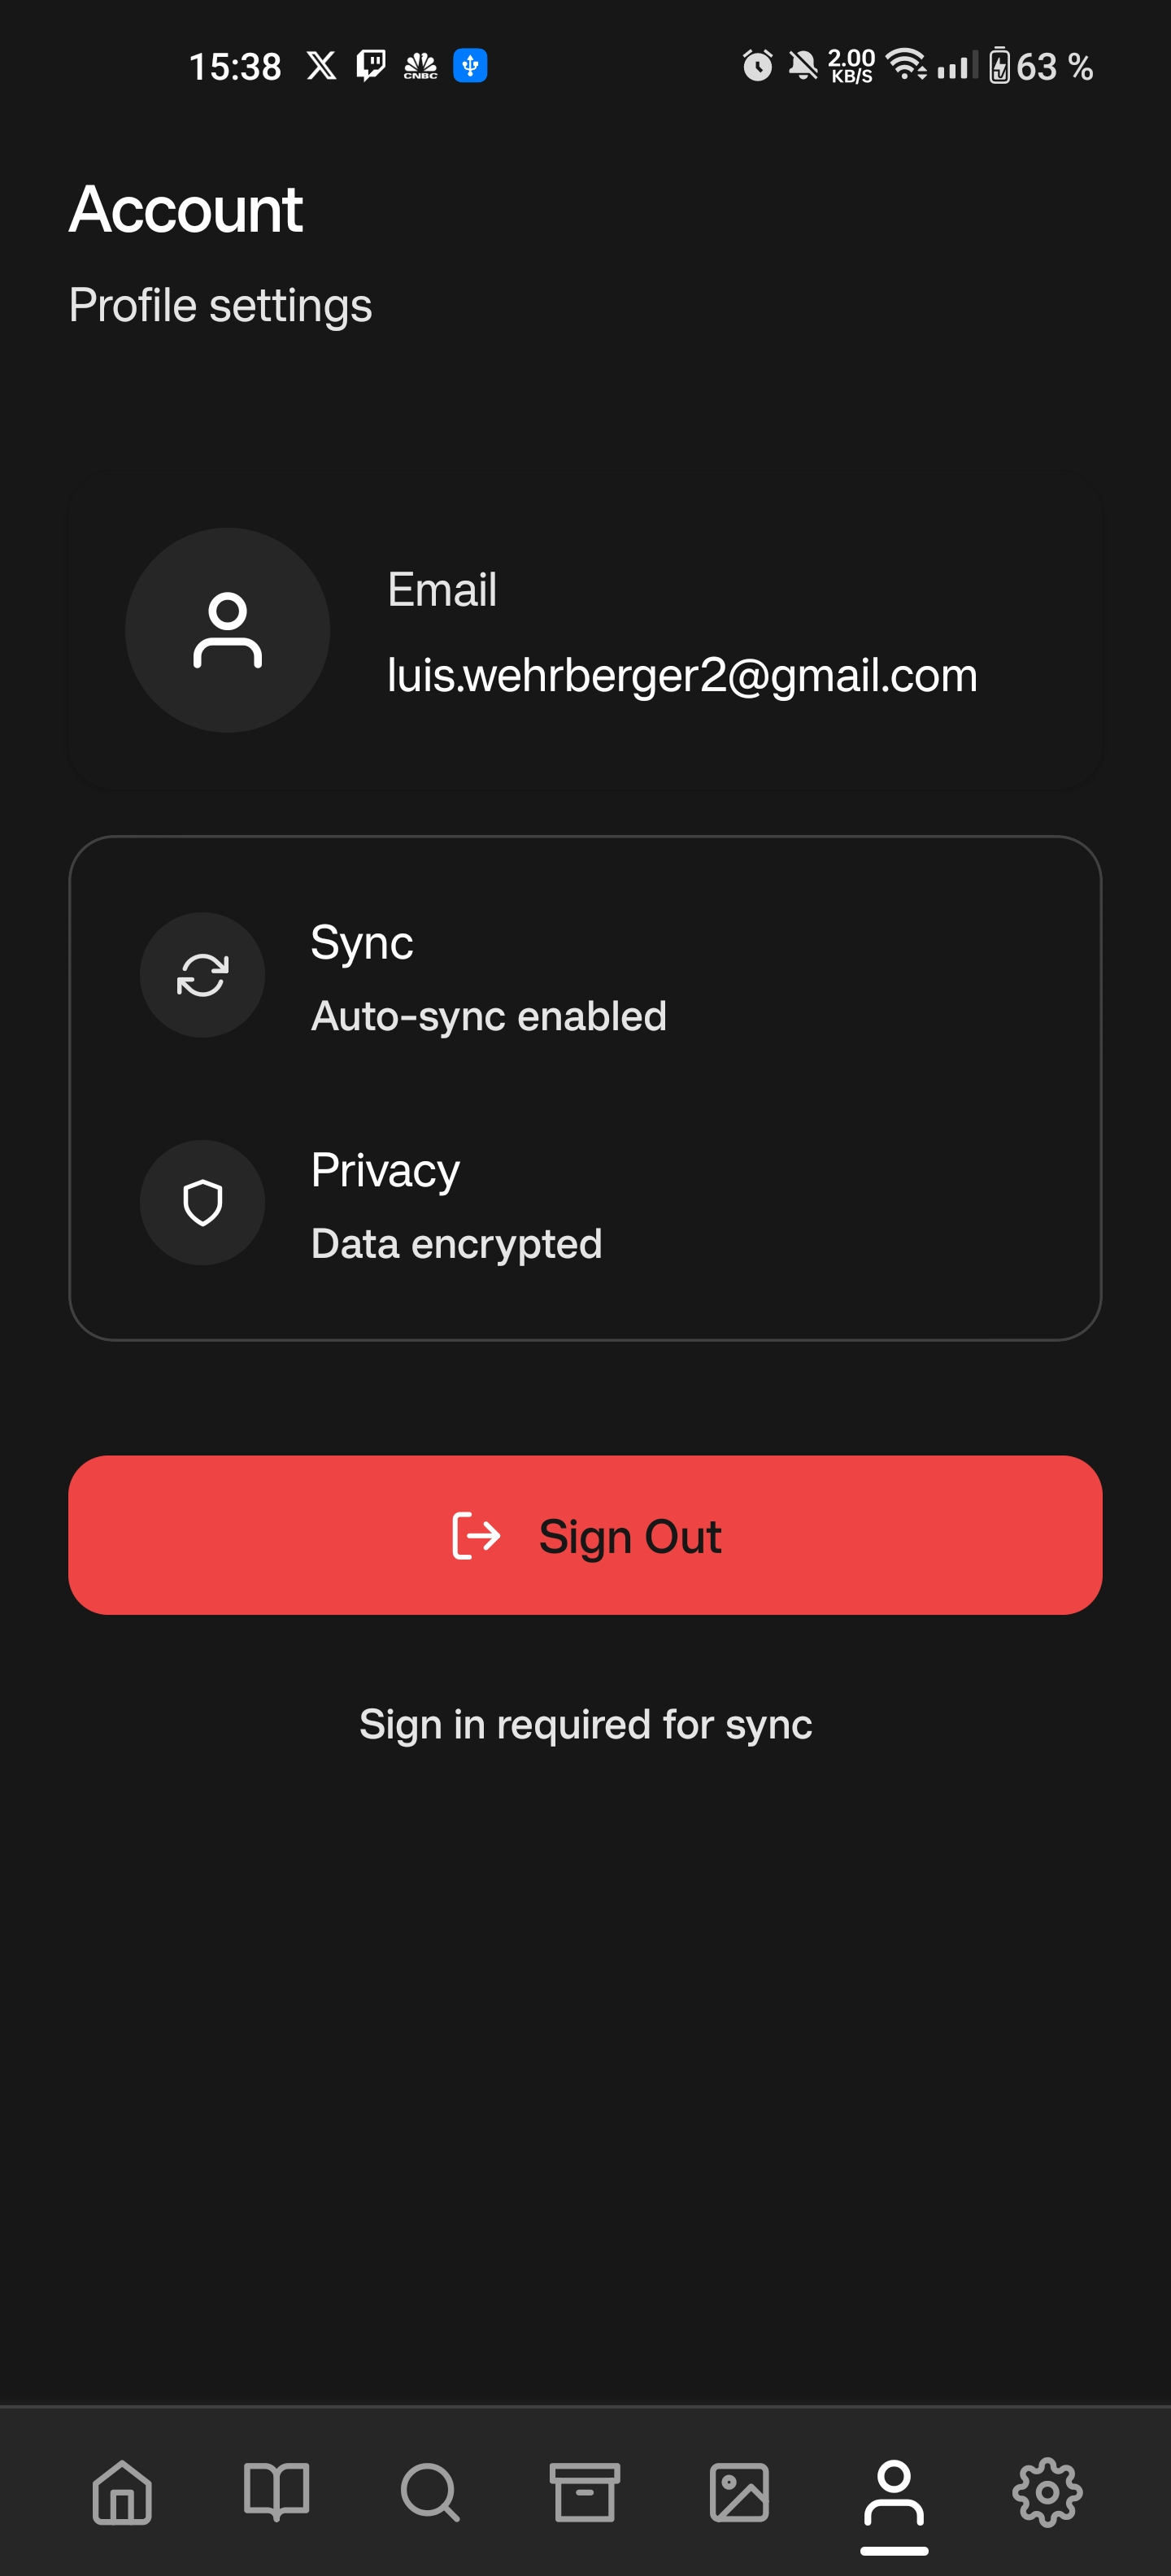
\includegraphics[width=\textwidth]{img/screenshots/account/main}
        \small{User profile and account management.}
    \end{minipage}
\end{figure}

\clearpage
\section{Feature Screens}

\subsection{Account Features}
The account section provides user authentication for syncing bird logs across devices. All other app features work completely offline without requiring login. This design ensures maximum accessibility while offering optional cloud synchronization for users who want to access their bird spotting data on multiple devices.

\begin{figure}[h]
    \centering
    \begin{minipage}[t]{0.3\textwidth}
        \centering
        \textbf{Login Screen}
        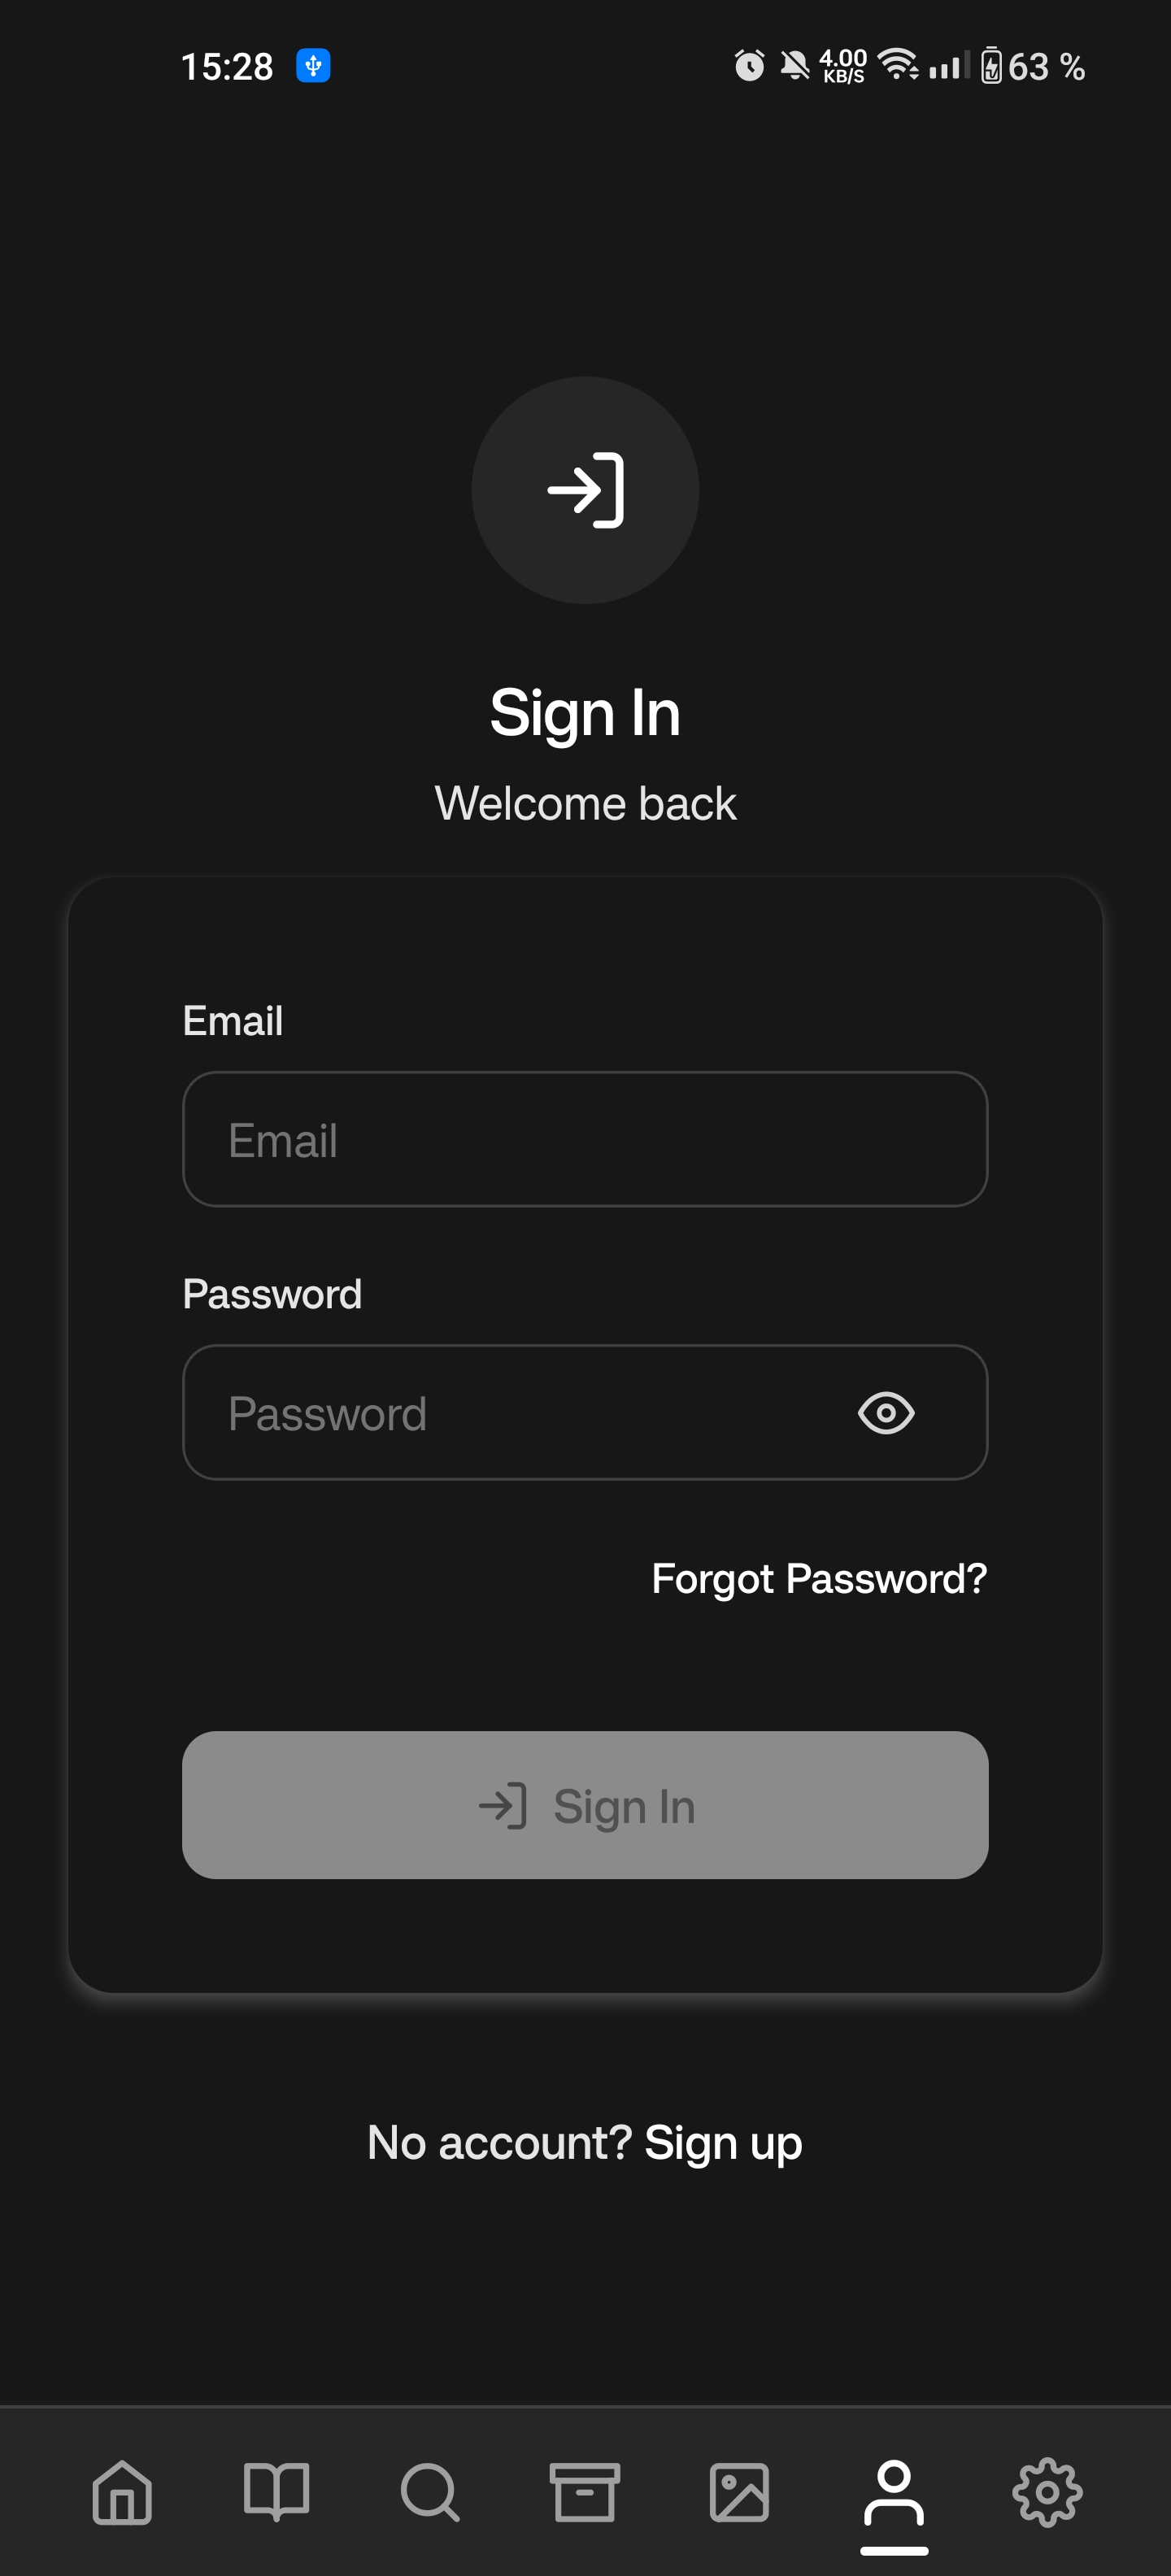
\includegraphics[width=\textwidth]{img/screenshots/account/login}
        \small{Optional login for cloud sync.}
    \end{minipage}%
    \hfill%
    \begin{minipage}[t]{0.3\textwidth}
        \centering
        \textbf{Profile Screen}
        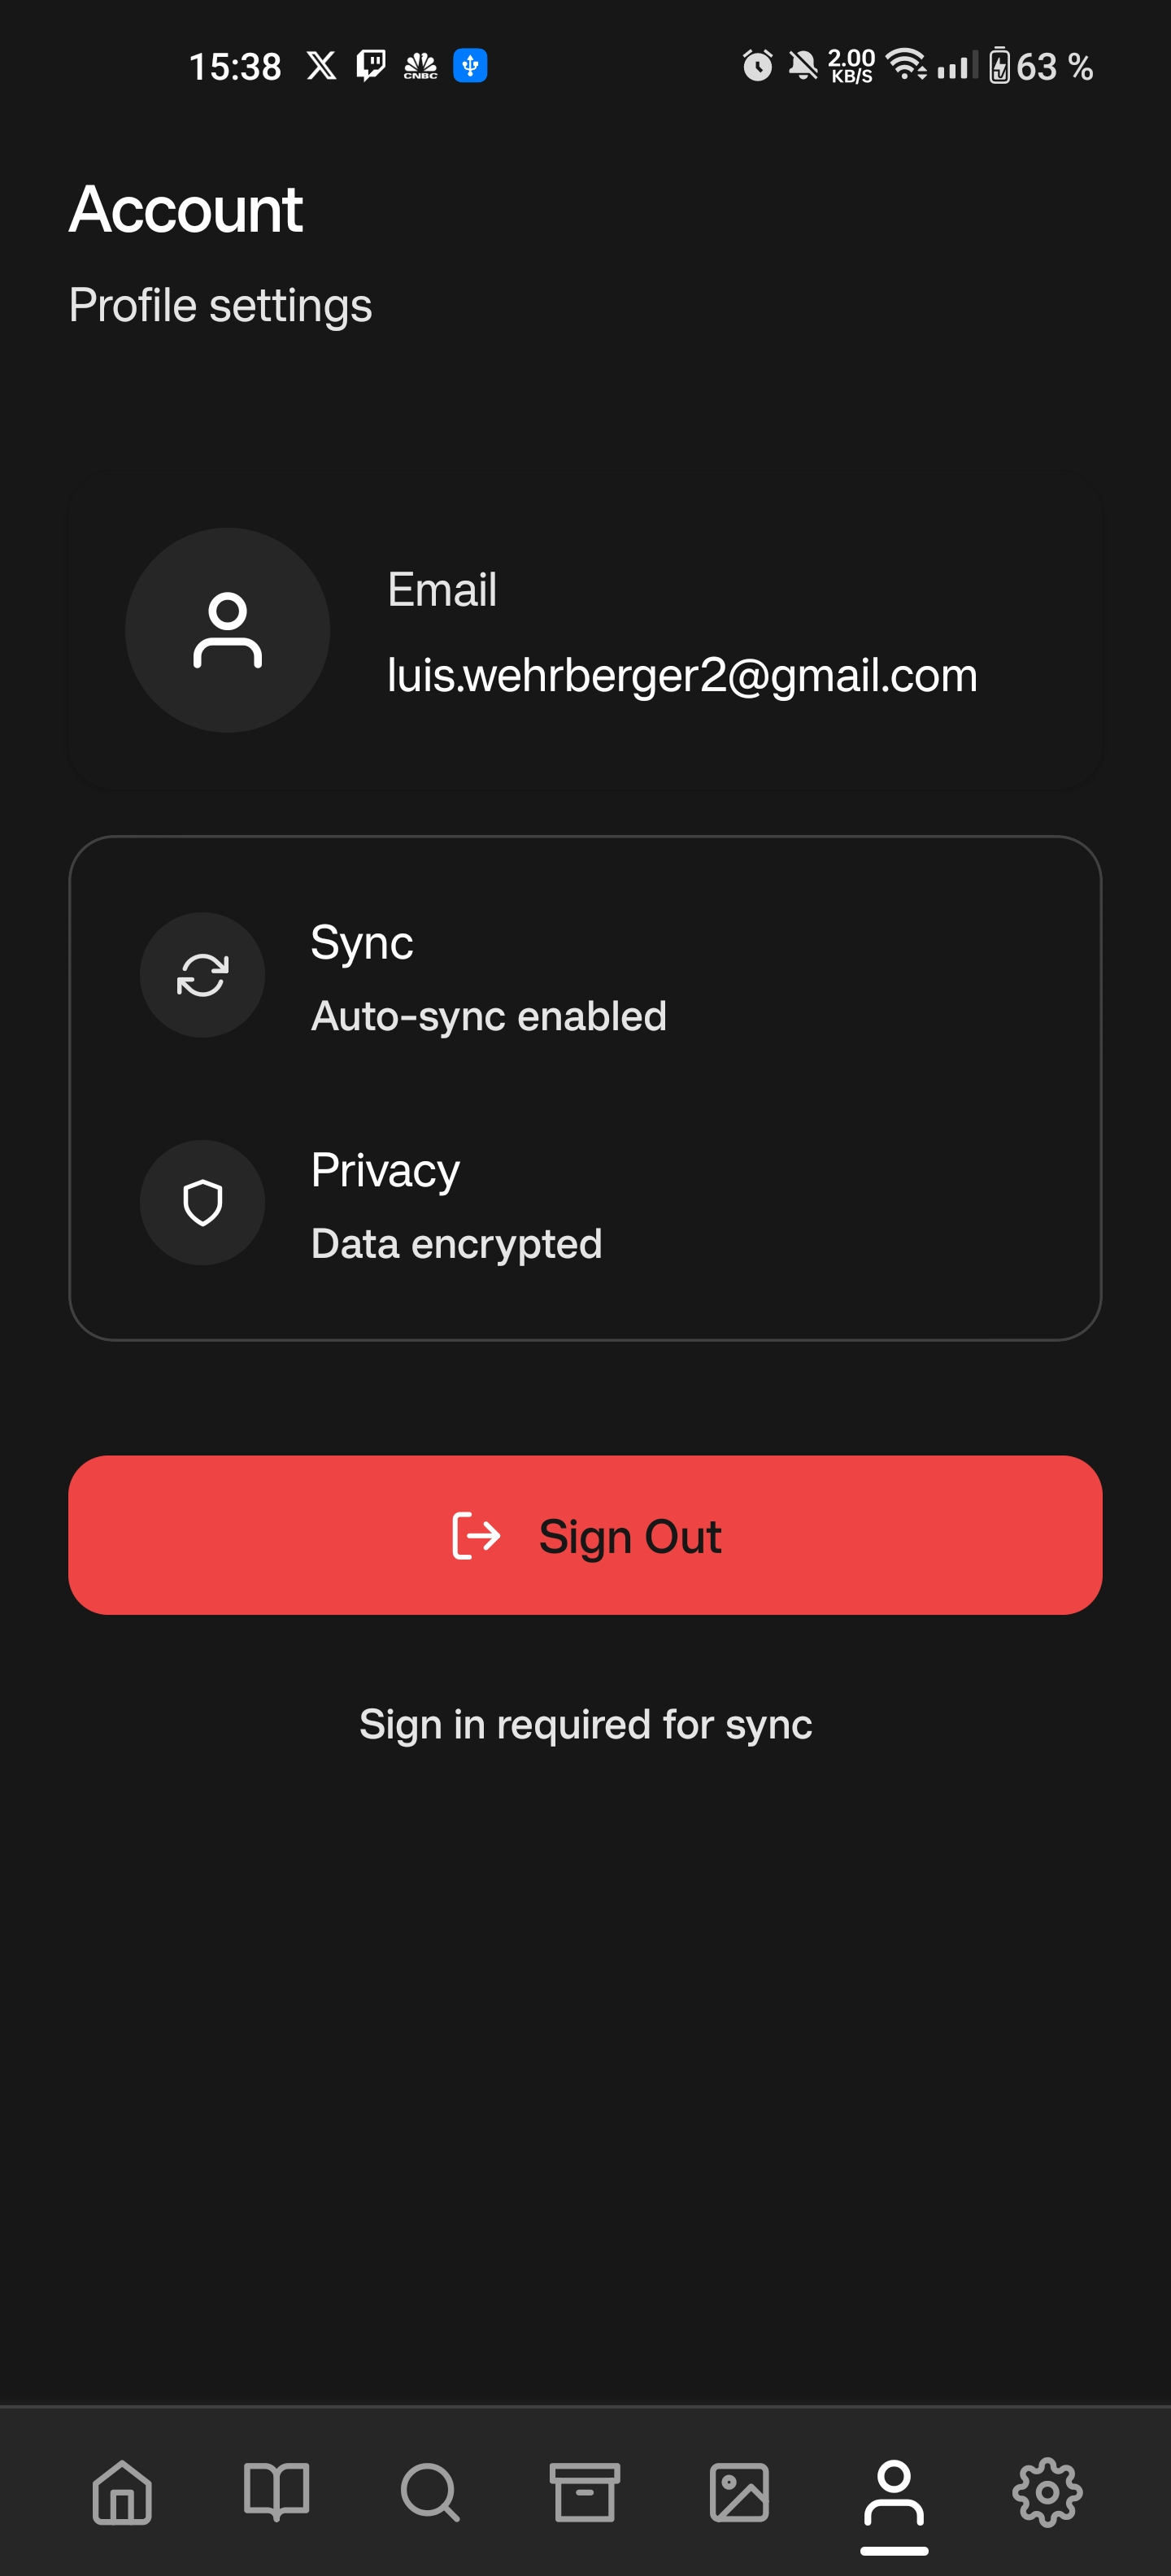
\includegraphics[width=\textwidth]{img/screenshots/account/main}
        \small{Sync status and settings.}
    \end{minipage}%
    \hfill%
    \begin{minipage}[t]{0.3\textwidth}
        \centering
        \textbf{Password Reset}
        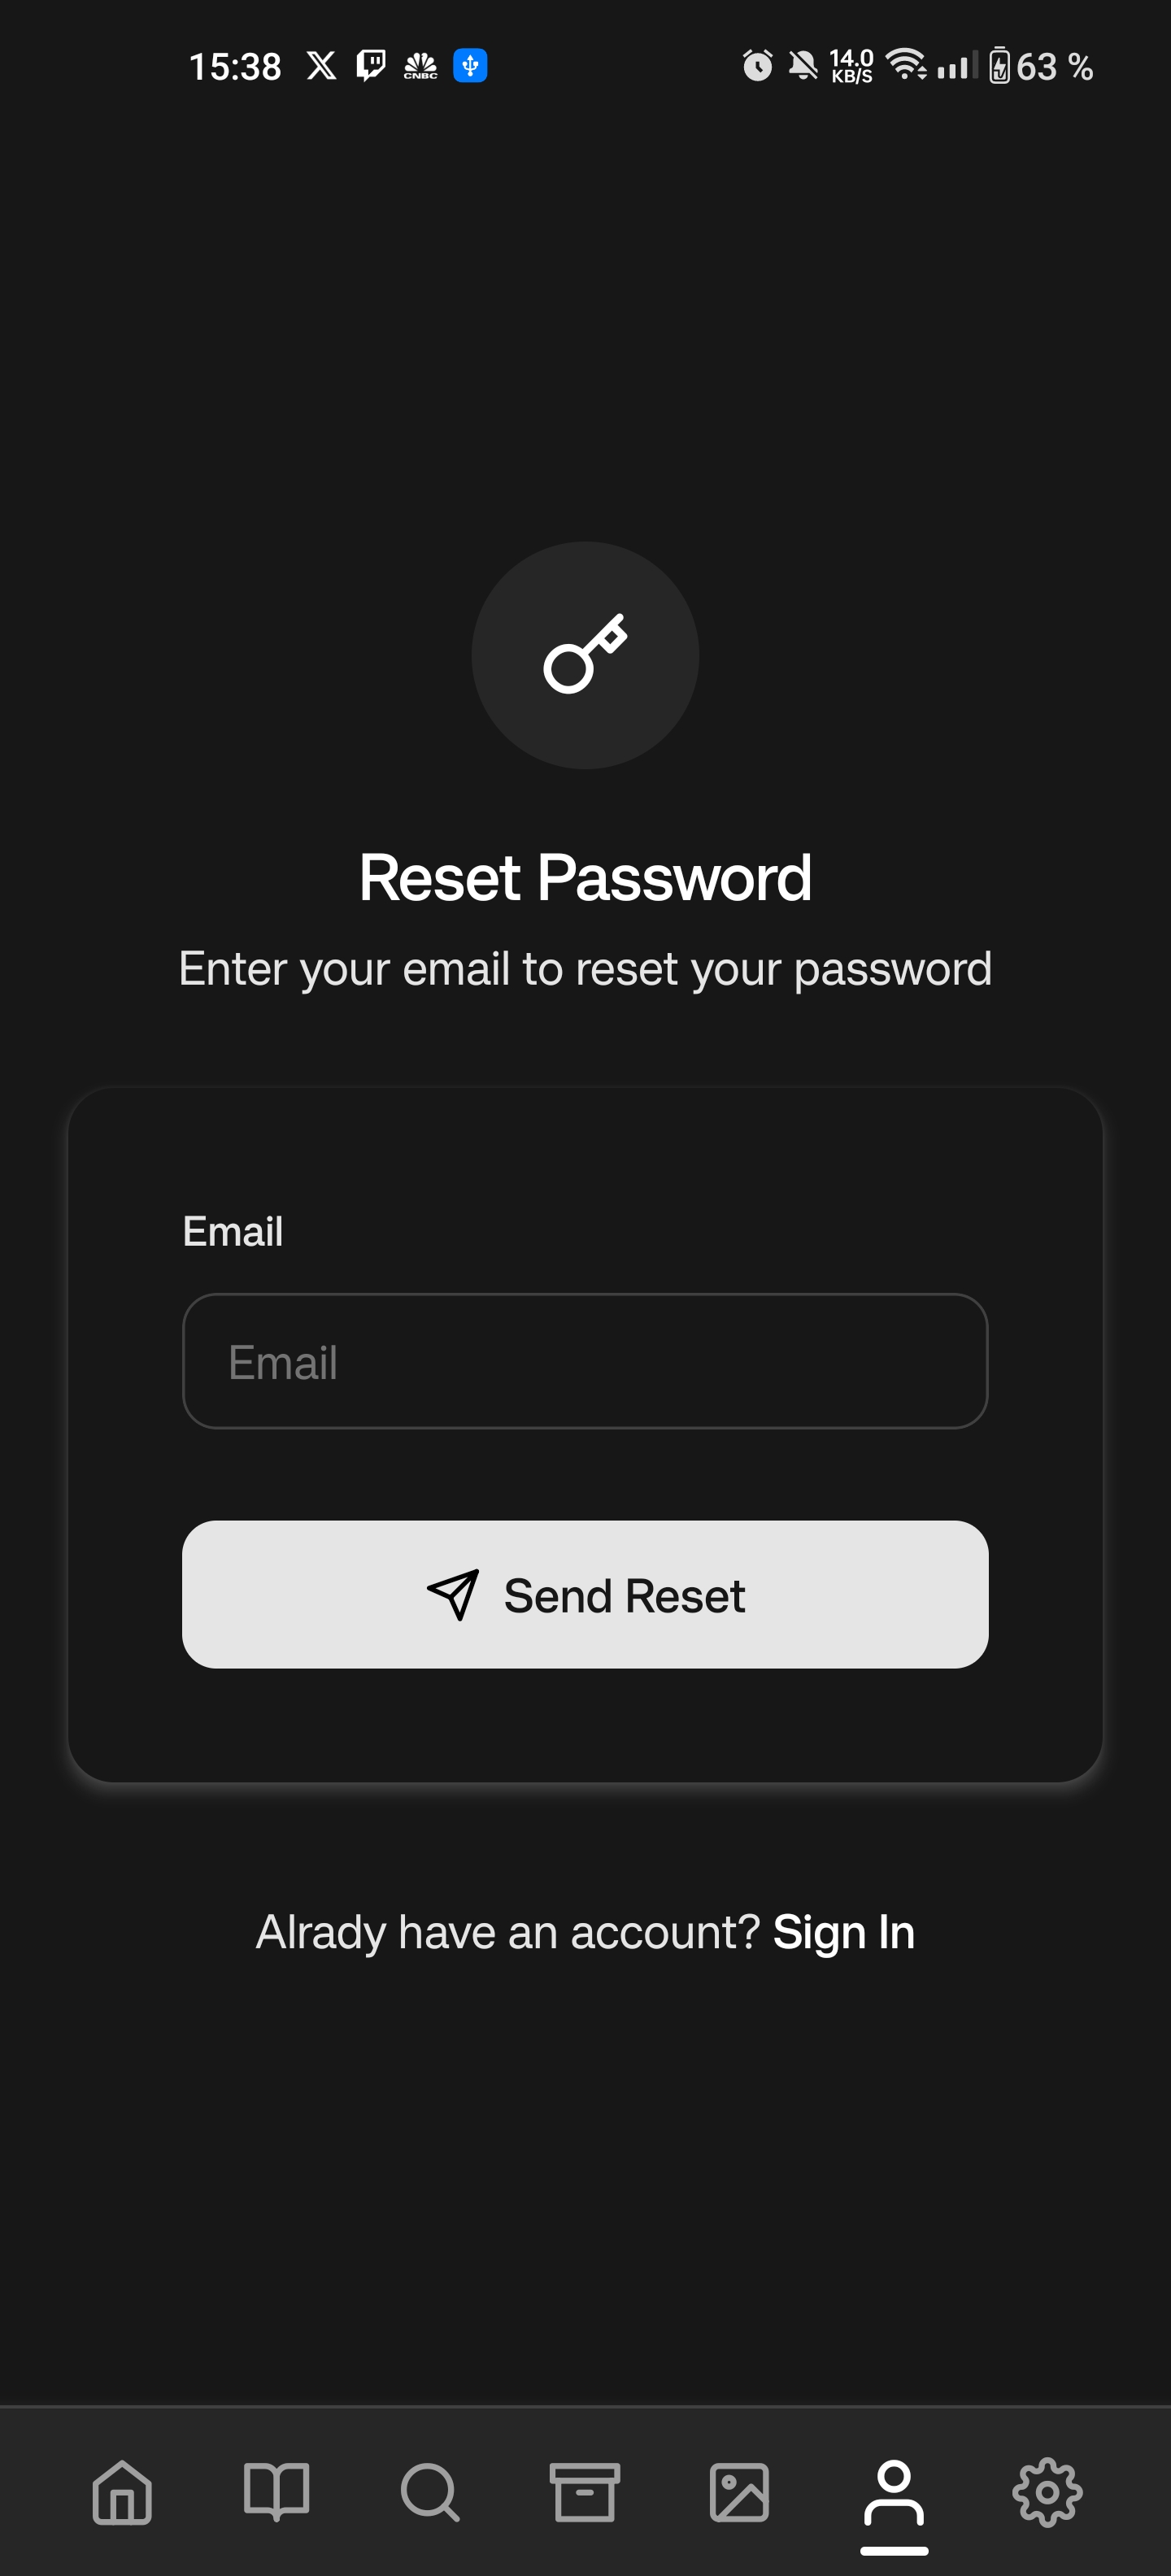
\includegraphics[width=\textwidth]{img/screenshots/account/reset_pw}
        \small{Account recovery for sync access.}
    \end{minipage}
\end{figure}

Key aspects of the account system:
\begin{itemize}
    \item \textbf{Optional Authentication}: Login is only required for cloud sync
    \item \textbf{Offline-First}: All features work without authentication, except sync
    \item \textbf{Sync Management}: Control when and how data syncs
    \item \textbf{Data Privacy}: Encrypted cloud storage when syncing
    \item \textbf{Cross-Device Access}: Access logs on multiple devices when logged in
\end{itemize}

\subsection{Logging Features}
The logging section offers various methods to record bird observations.

\begin{figure}[h]
    \centering
    \begin{minipage}[t]{0.3\textwidth}
        \centering
        \textbf{Manual Log}
        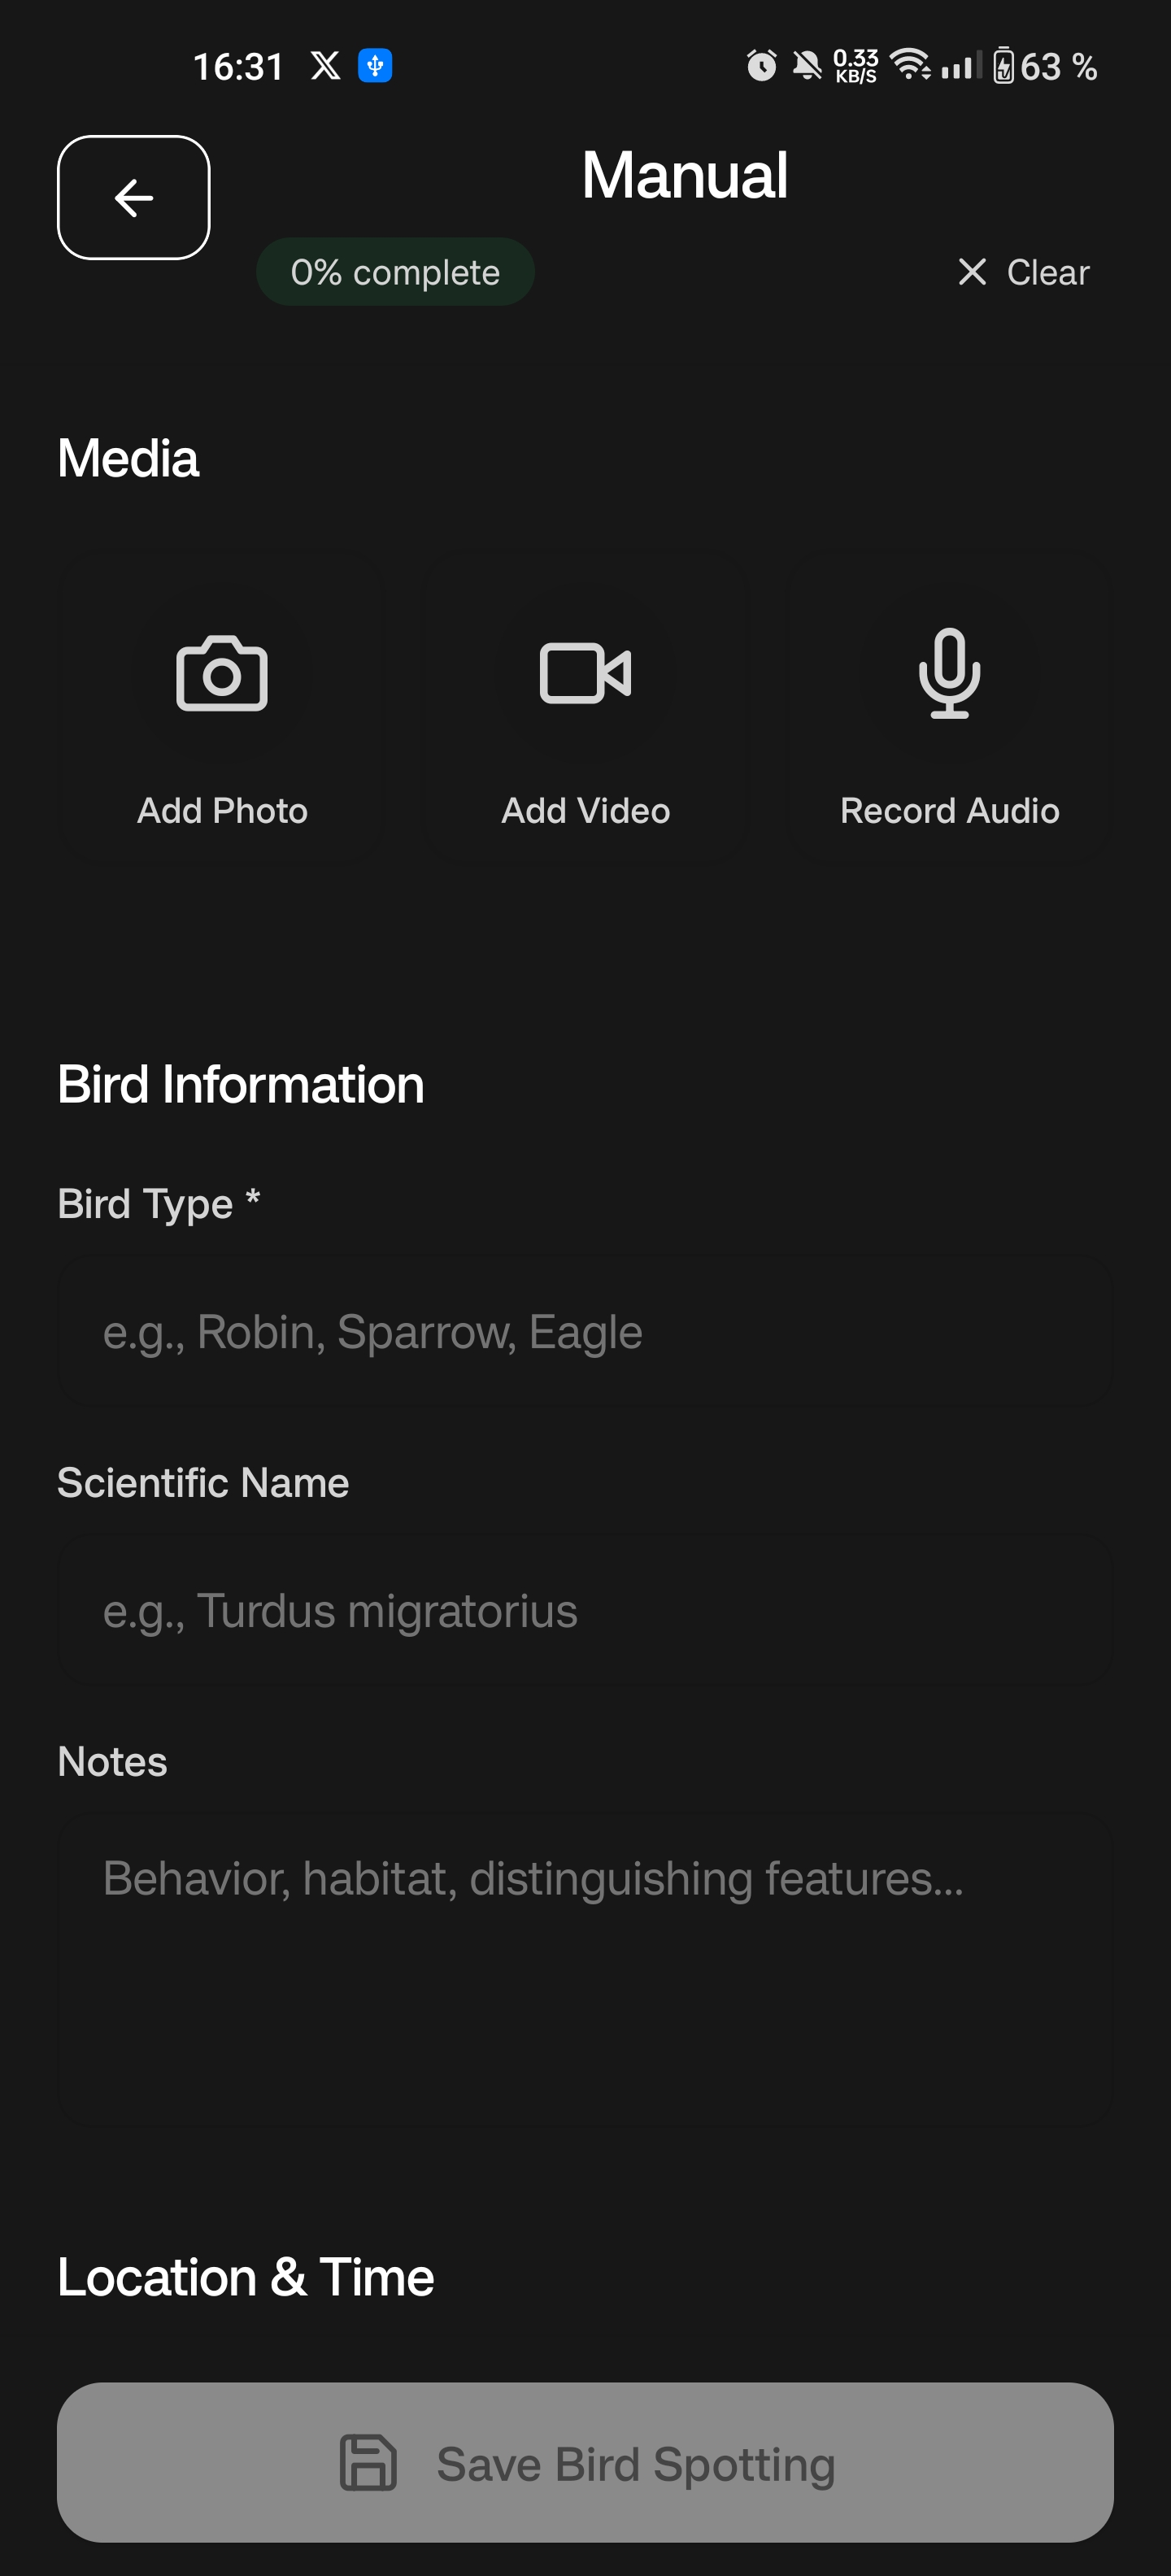
\includegraphics[width=\textwidth]{img/screenshots/log/manual}
        \small{Manual bird observation entry.}
    \end{minipage}%
    \hfill%
    \begin{minipage}[t]{0.3\textwidth}
        \centering
        \textbf{Audio Recording}
        
\includegraphics[width=\textwidth]{img/screenshots/log/audio}
        \small{Bird song recording interface.}
    \end{minipage}%
    \hfill%
    \begin{minipage}[t]{0.3\textwidth}
        \centering
        \textbf{Photo Logging}
        
\includegraphics[width=\textwidth]{img/screenshots/log/photo}
        \small{Photo-based bird logging.}
    \end{minipage}
\end{figure}

\begin{figure}[h]
    \centering
    \begin{minipage}[t]{0.3\textwidth}
        \centering
        \textbf{Auto Identification}
        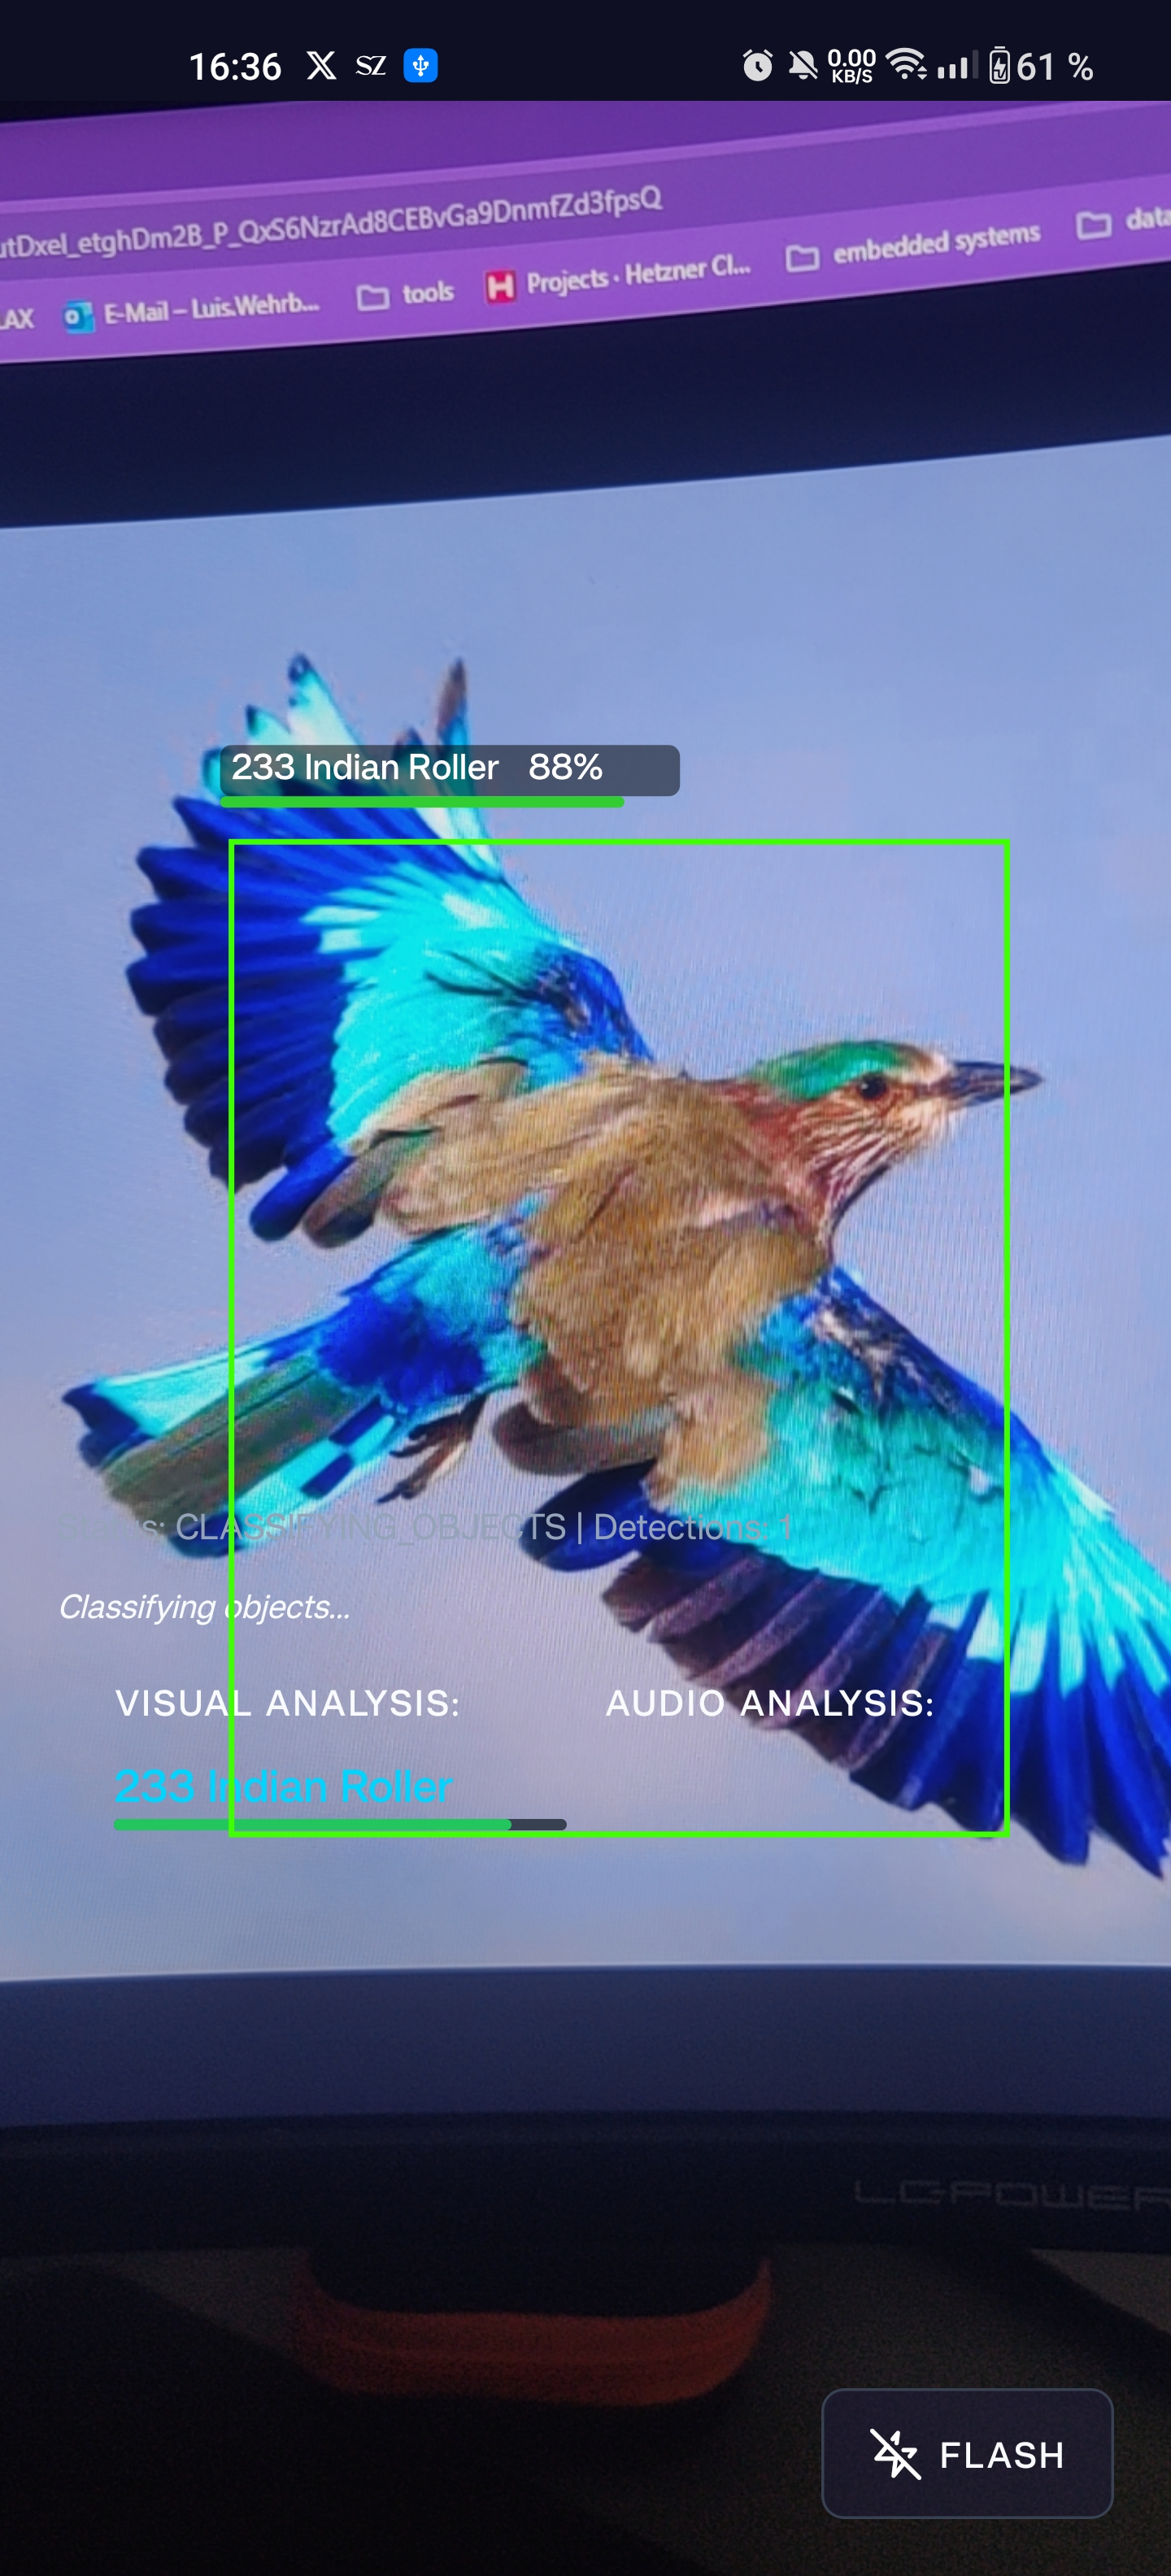
\includegraphics[width=\textwidth]{img/screenshots/log/auto_ident}
        \small{AI-powered bird identification.}
    \end{minipage}
\end{figure}

\subsection{Archive Features}
The archive section provides comprehensive management of past observations.

\begin{figure}[h]
    \centering
    \begin{minipage}[t]{0.3\textwidth}
        \centering
        \textbf{Sort View}
        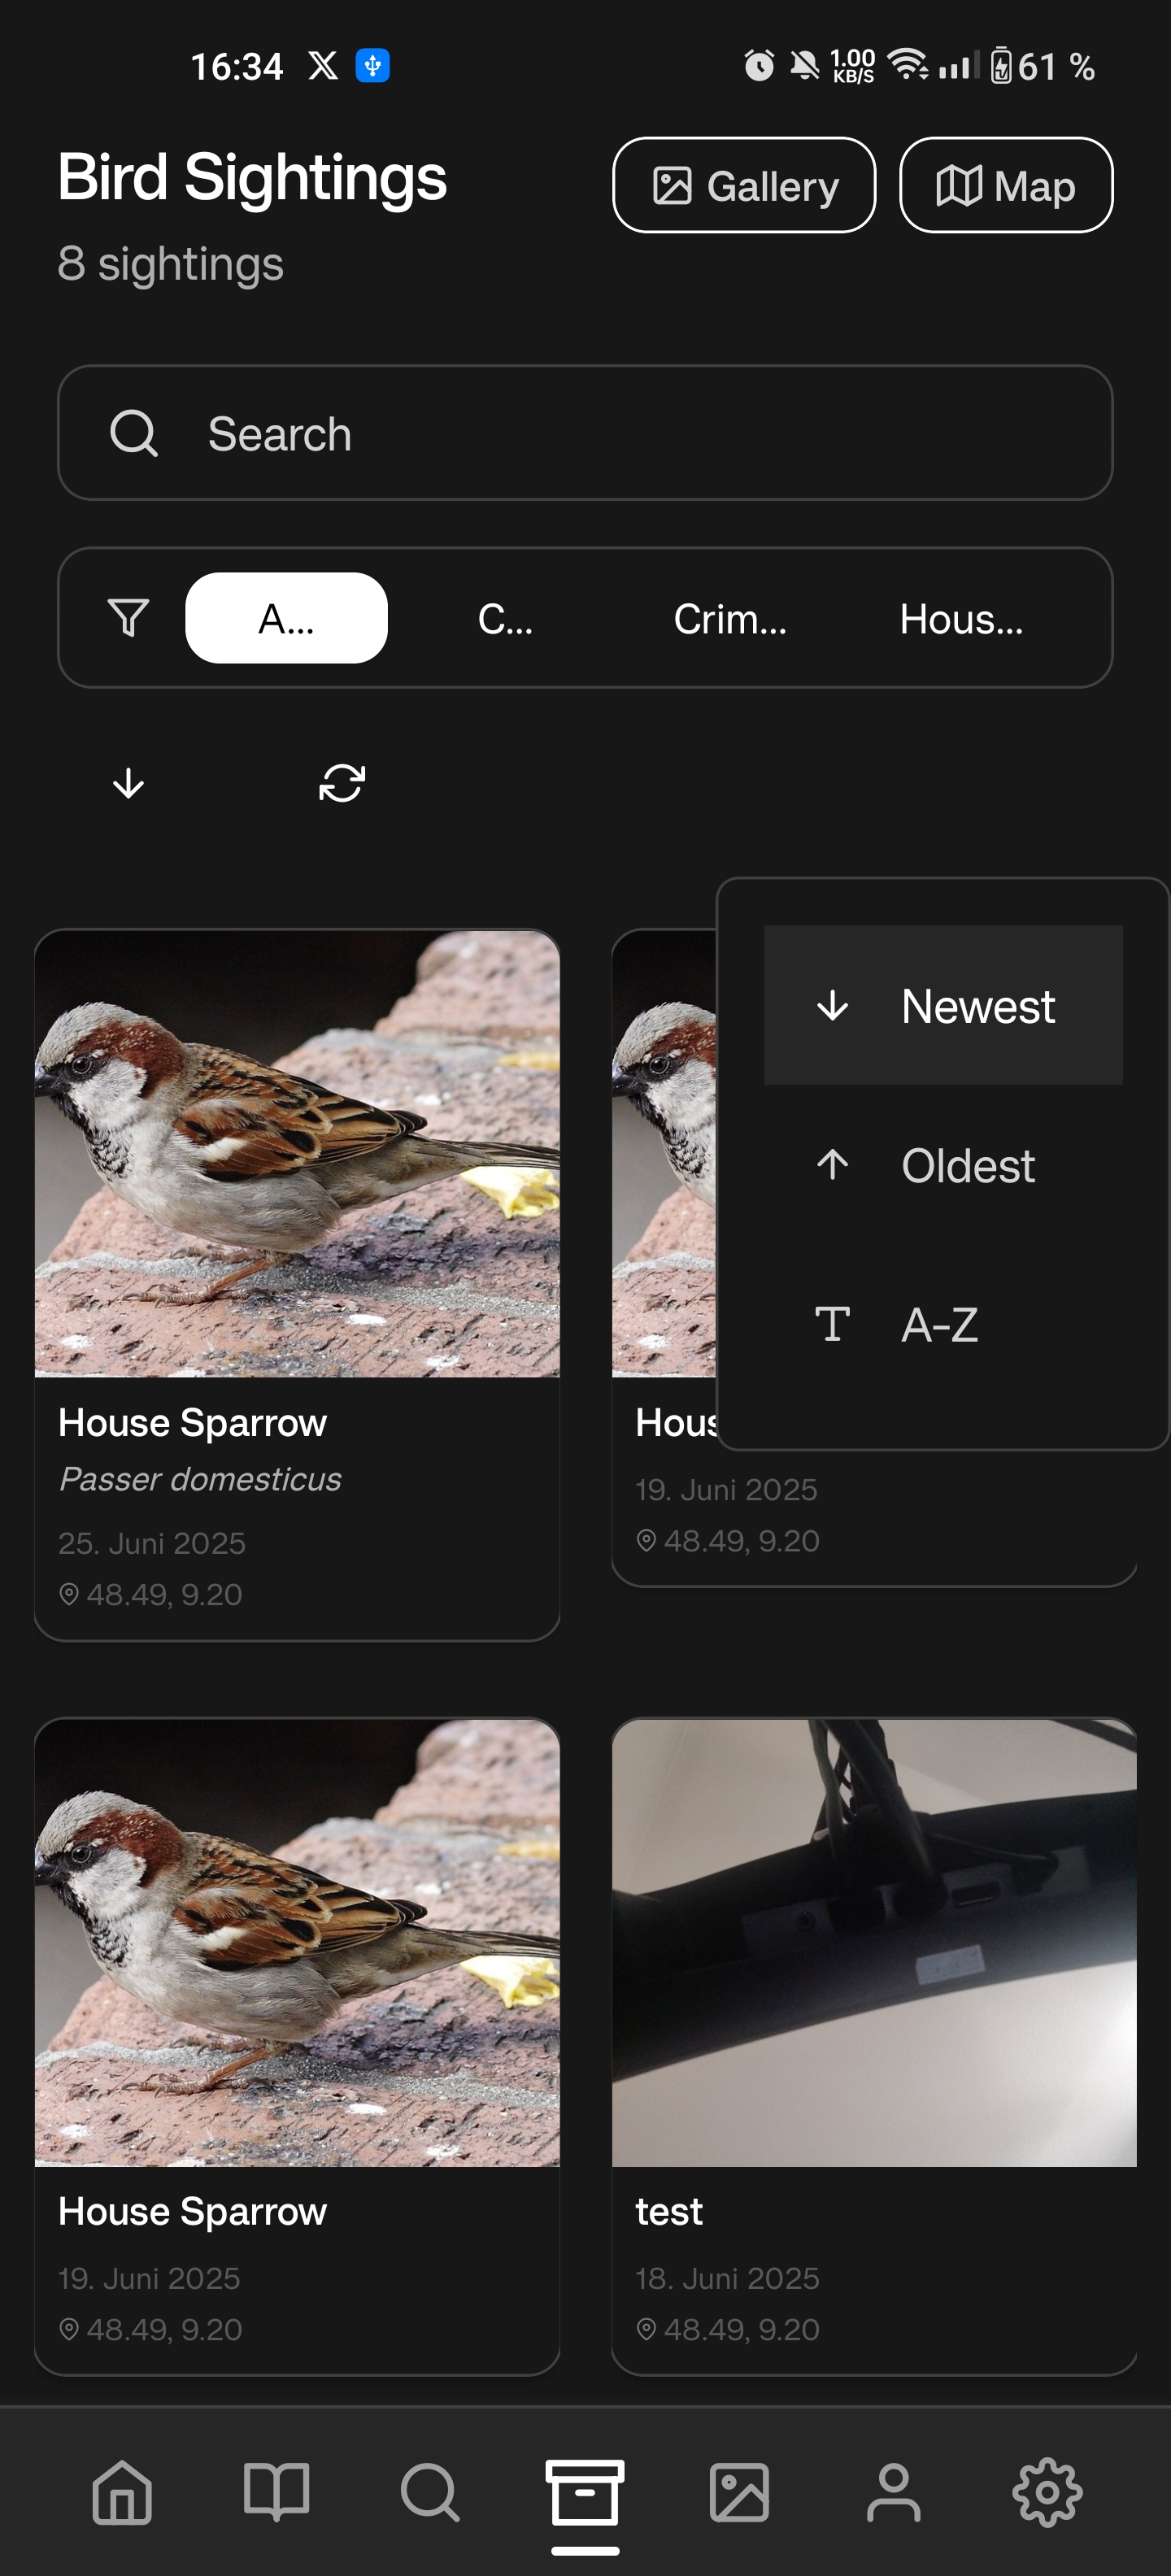
\includegraphics[width=\textwidth]{img/screenshots/archive/sort}
        \small{Sorting and filtering options.}
    \end{minipage}%
    \hfill%
    \begin{minipage}[t]{0.3\textwidth}
        \centering
        \textbf{Map Overview}
        \includegraphics[width=\textwidth]{img/screenshots/archive/big_map}
        \small{Geographical view of observations.}
    \end{minipage}%
    \hfill%
    \begin{minipage}[t]{0.3\textwidth}
        \centering
        \textbf{Sync Progress}
        \includegraphics[width=\textwidth]{img/screenshots/archive/sync_on_going}
        \small{Data synchronization status.}
    \end{minipage}
\end{figure}

\begin{figure}[h]
    \centering
    \begin{minipage}[t]{0.3\textwidth}
        \centering
        \textbf{Sync Complete}
        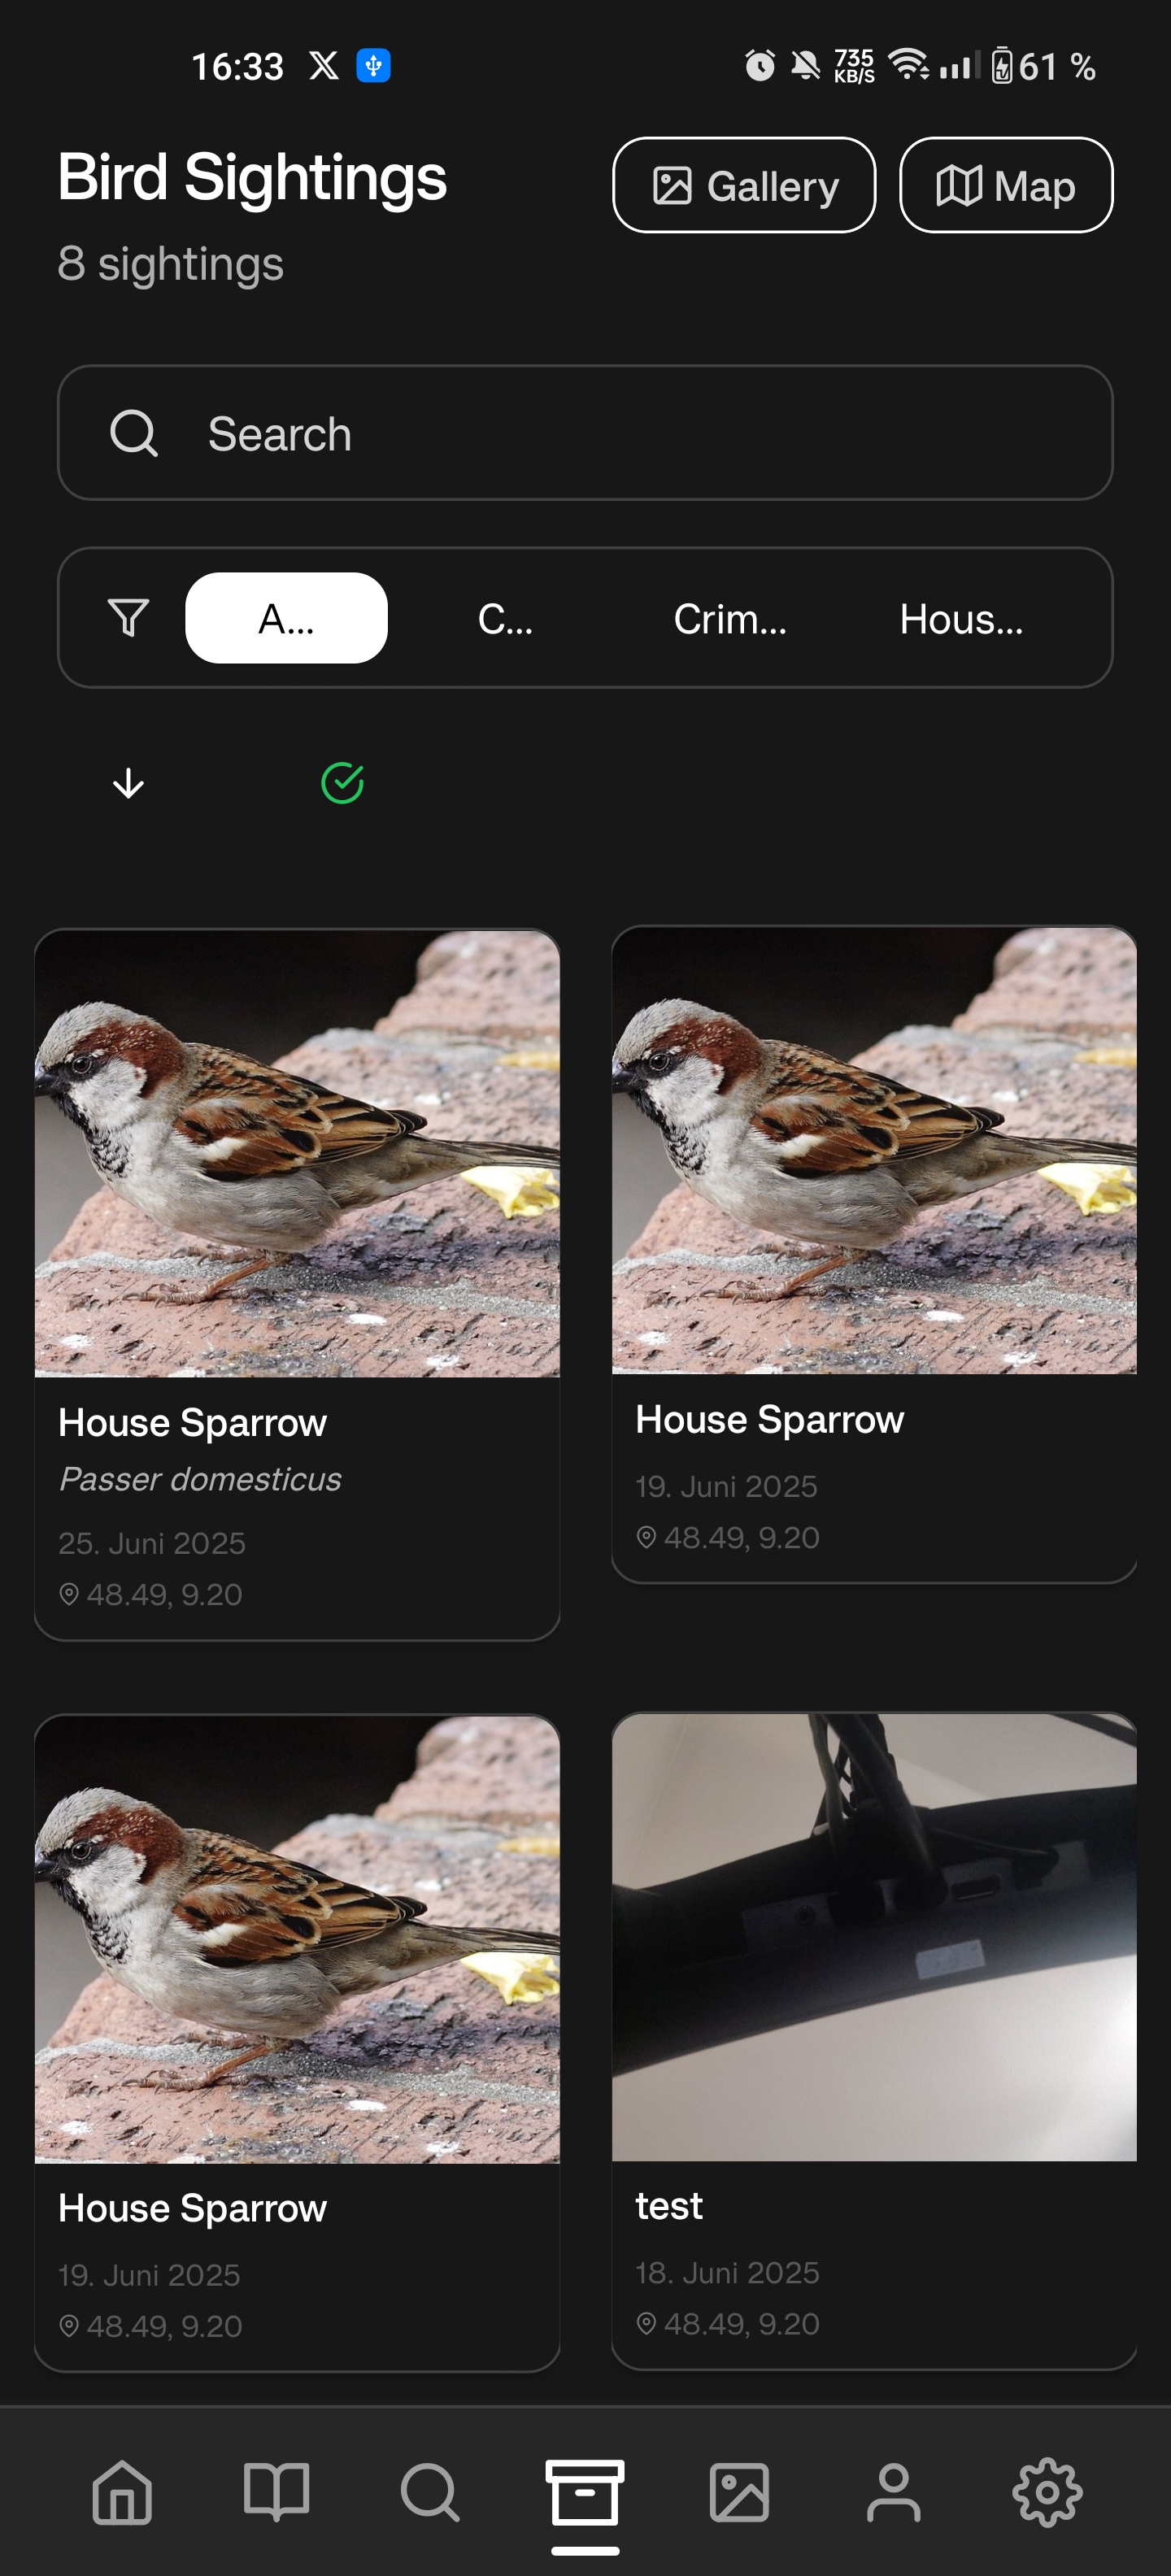
\includegraphics[width=\textwidth]{img/screenshots/archive/sync_done}
        \small{Successful synchronization view.}
    \end{minipage}
\end{figure}

\subsection{BirdDex Features}
The BirdDex section provides comprehensive bird species information and sorting capabilities.

\begin{figure}[h]
    \centering
    \begin{minipage}[t]{0.3\textwidth}
        \centering
        \textbf{Sort by Attribute}
        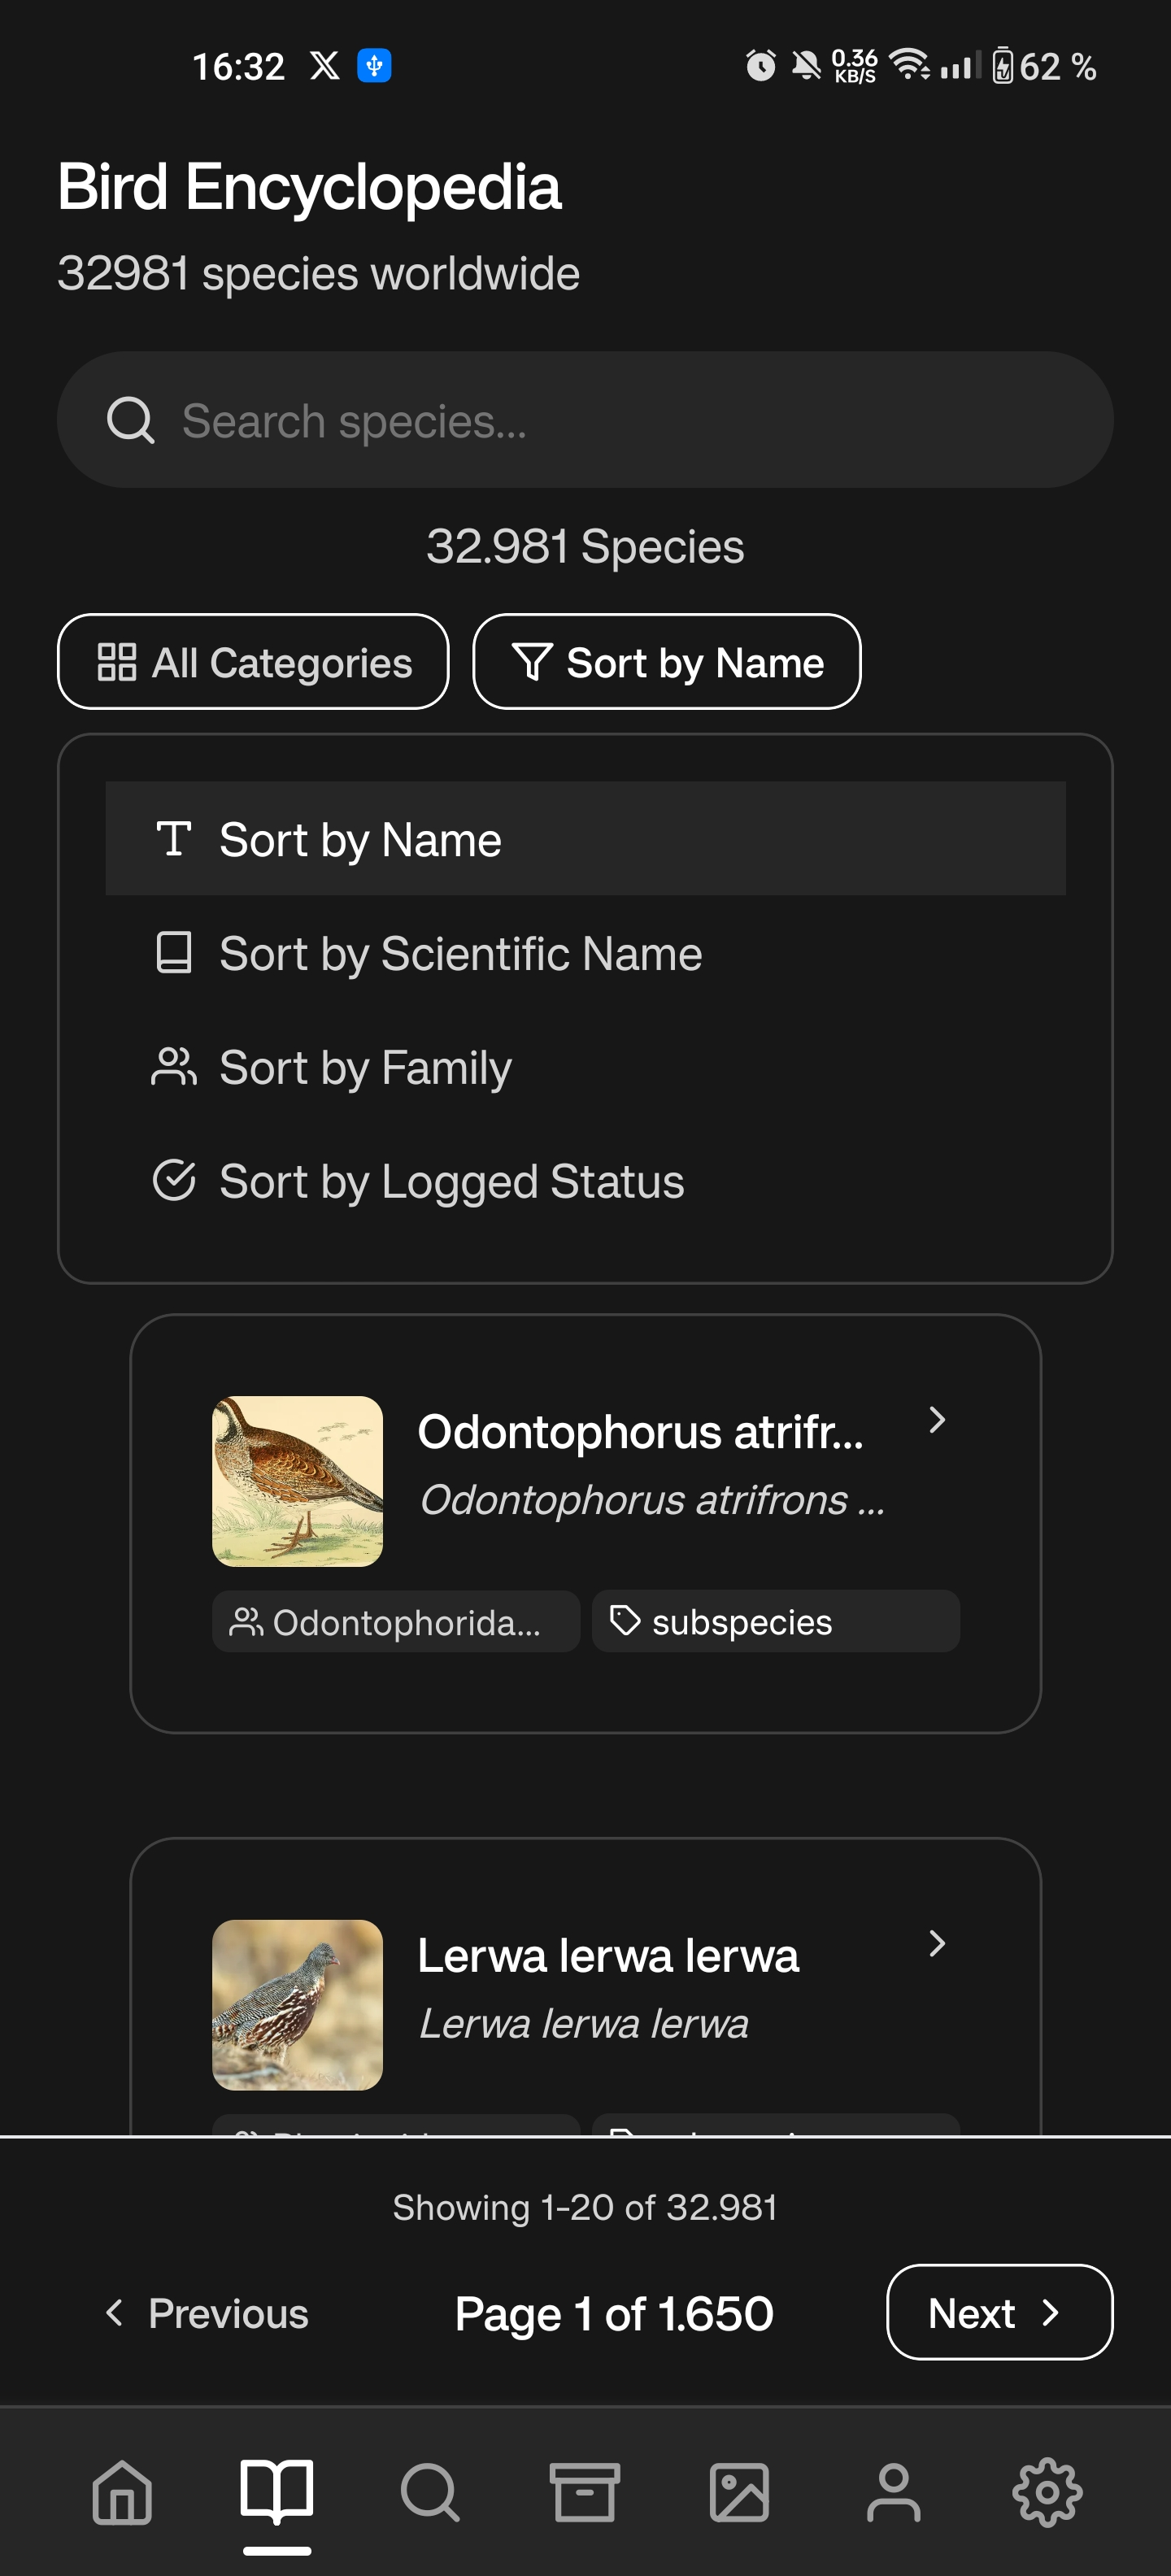
\includegraphics[width=\textwidth]{img/screenshots/bird_dex/sort_by_attribute}
        \small{Attribute-based species sorting.}
    \end{minipage}%
    \hfill%
    \begin{minipage}[t]{0.3\textwidth}
        \centering
        \textbf{Sort by Category}
        \includegraphics[width=\textwidth]{img/screenshots/bird_dex/sort_by_category}
        \small{Category-based species organization.}
    \end{minipage}
\end{figure}



\end{document}